\documentclass[11pt,a4paper]{article}
\usepackage[margin=2.3cm]{geometry}
\usepackage[T1]{fontenc}
\usepackage{lmodern}
\usepackage{microtype}
\usepackage{amsmath,amssymb}
\usepackage{graphicx}
\usepackage{booktabs}
\usepackage{caption}
\usepackage{float}
\usepackage{xcolor}
\usepackage[hidelinks]{hyperref}
\captionsetup{font=small,labelfont=bf}
\graphicspath{{../figures/}}
\setlength{\parskip}{0.35em}
% Let large figures share pages with text instead of sitting alone on
% half-empty float pages.
\renewcommand{\topfraction}{0.9}
\renewcommand{\bottomfraction}{0.8}
\renewcommand{\textfraction}{0.07}
\renewcommand{\floatpagefraction}{0.8}
\setcounter{topnumber}{3}
\setcounter{totalnumber}{5}
\title{Machine-Learning Screening of Electrocatalytic 5-Hydroxymethylfurfural
Oxidation to 2,5-Furandicarboxylic Acid from Literature Data: Leakage-Aware Classification,
Regression and Multi-Objective Optimisation}
\author{\textit{Author names and affiliations to be added}}
\date{11 November 2026}
\begin{document}
\maketitle
\begin{abstract}
We assembled 154 electrocatalytic HMF-oxidation records from 99 publications and built a leakage-aware machine-learning pipeline that (i) engineers chemical descriptors for the catalyst, electrolyte, cell configuration and operating conditions, (ii) clusters reported conversion and FDCA yield with K-means, (iii) compares six classifier families under four class-balancing strategies, (iv) interprets the selected models with SHAP, (v) regresses four performance outcomes and (vi) searches catalyst/condition space with a validation-gated NSGA-II. All model selection uses publication-grouped cross-validation so that no paper contributes records to both training and test folds. Correcting descriptor extraction (anode-only catalyst parsing, formula-aware compound families, temperature and pH parsing, counter-electrode descriptors), retaining missing-value indicators and re-tuning the models raised the best pooled out-of-fold macro-F1 for a binary $\geq$90\% performance screen from 0.586 to 0.731 (neural network with SMOTE; 95\% CI 0.717--0.744; stratified dummy 0.480), and for three-cluster K-means labels from 0.421 to 0.626. We also identify and correct an evaluation flaw in which folds where an oversampler could not be fitted were silently discarded, which had inflated earlier $K=4$ scores. No model--sampler combinations reached a mean macro-F1 of 0.76, reflecting the small, heterogeneous and imbalanced literature corpus rather than a pipeline limitation. Regression models only modestly beat a median baseline, and NSGA-II outputs are presented as hypotheses for experimental testing.
\end{abstract}
\noindent\textbf{Keywords:} HMF electrooxidation; FDCA; machine learning; grouped cross-validation; class imbalance; SHAP; NSGA-II

\section{Introduction}
2,5-Furandicarboxylic acid (FDCA) is a bio-based replacement for terephthalic acid, and its
electrochemical production from 5-hydroxymethylfurfural (HMF) couples biomass valorisation with
renewable electricity. Reported performance depends jointly on the anode material, electrolyte,
applied potential, temperature, mediator use and cell design, and the published literature now
contains enough individual experiments to attempt data-driven screening. Literature-mined
datasets are, however, small, heterogeneously reported and dominated by high-performing results,
which makes naive machine-learning evaluation prone to optimistic bias: records from the same
paper share catalysts and protocols, so random cross-validation leaks information between
training and test sets.

Following the integrated workflow of Li \textit{et al.}~\cite{li2025}, which combined K-means
labelling, oversampling, classifier comparison, SHAP interpretation and a genetic algorithm for
thermal aerobic HMF oxidation, we adapt the methodology to electro-oxidation and make three
contributions: (1) a publication-grouped, fold-local evaluation protocol in which imputation,
scaling and oversampling are fitted only on training papers; (2) a corrected descriptor set for
the anode catalyst, electrolyte and cell configuration; and (3) an honest assessment of how far
classification, regression and optimisation can be pushed with the current corpus.
\section{Data and methods}
\subsection{Literature dataset}
The corpus contains 154 experiments from 99 publications (Table~\ref{tab:data}). Each record lists the cell type, HMF concentration, catalyst description, electrolyte, applied potential, TEMPO use, temperature and up to four outcomes: HMF conversion, FDCA yield, faradaic efficiency (FE) and selectivity. Outcome reporting is incomplete; only 60 records report all four outcomes.

\begin{table}[!htbp]
\centering
\caption{Dataset composition. Missing counts per continuous descriptor: \texttt{Temperature\_C} (63), \texttt{Potential\_vs\_RHE\_V} (32), \texttt{Electrolyte\_Concentration\_M} (10), \texttt{HMF\_Concentration\_mM} (6), \texttt{Electrolyte\_pH} (2).}
\label{tab:data}
\begin{tabular}{lr}
\toprule
Quantity & Value \\
\midrule
Literature records & 154 \\
Independent publications (CV groups) & 99 \\
Input descriptors (before missing-value indicators) & 61 \\
Missing-value indicator columns added in-fold & 5 \\
Records reporting conversion & 117 \\
Records reporting FDCA yield & 123 \\
Records reporting faradaic efficiency & 119 \\
Records reporting selectivity & 91 \\
Records reporting all four outcomes & 60 \\
Binary-screen records (FDCA product, yield reported) & 119 (89 positive) \\
\bottomrule
\end{tabular}
\end{table}
\subsection{Descriptor engineering}
Inputs are restricted to eight agreed experimental groups: TEMPO, temperature, reactant,
HMF concentration, catalyst, electrolyte, potential versus RHE and cell configuration. All
measured outcomes and any column derived from them are excluded. Three corrections to the
earlier descriptor extraction were made in this revision.
\begin{itemize}
\item \textbf{Anode-only catalyst parsing.} Catalyst strings describe the whole cell
(e.g.\ ``Anode: Ni$_3$N@C on Ni foam. Cathode: Pt foil''). The previous parser searched the full
string, so 74 records were flagged as Pt catalysts because of the Pt counter electrode. Element
and compound flags are now extracted from the anode/working-electrode segment only, which leaves
2 genuine Pt anodes.
\item \textbf{Formula-aware compound families.} Phosphide, nitride, sulfide and selenide
flags had been matched only on words such as ``phosphide'' and were zero for every record.
Case-sensitive formula patterns (Ni$_3$S$_2$, CoNiP, VN, Co$_9$S$_8$, Ni$_2$P) now recover 12
phosphide, 8 nitride and 15 sulfide anodes, plus borides, foam substrates, conductive supports
(FTO, ITO, BDD), element counts, a noble-metal flag and a bimetallic flag.
\item \textbf{Operating conditions.} ``23 $\pm$ 2\,$^\circ$C'' had been parsed as 2\,$^\circ$C;
uncertainties are now stripped first. An electrolyte pH is taken from explicit ``pH'' values or
inferred as $14+\log_{10}[\mathrm{OH^-}]$ for hydroxides. Counter-electrode descriptors
(Pt, carbon, Ni, reported) are added to the cell-configuration group.
\end{itemize}
This yields 61 descriptors. Within every training fold, missing continuous values are median-imputed and a binary indicator is appended for each of the 5 descriptors with missing values. Whether a paper reports, for example, its temperature or potential is a property of the input record and carries information that median imputation alone would erase.
\subsection{Classification targets}
\textit{K-means labels.} Conversion and FDCA yield are standardised and clustered for
$K\in\{3,4,5,6\}$ (100 initialisations). Missing outcomes are median-imputed for clustering only
and flagged; labels are never used as inputs (Table~\ref{tab:clusters}).

\textit{Binary performance screen.} For records whose major product is FDCA and whose yield is
reported, a performance score
\begin{equation}
P = \begin{cases} \min(X, Y) & \text{if conversion } X \text{ is reported,}\\ Y & \text{otherwise,}\end{cases}
\end{equation}
is computed from conversion $X$ and yield $Y$, and records with $P\geq 90\%$ form the positive class.
\begin{table}[!htbp]
\centering
\caption{K-means cluster sizes on (conversion, FDCA yield). The minority clusters are extremely small, which bounds the attainable macro-F1 under publication-grouped validation.}
\label{tab:clusters}
\begin{tabular}{rlr}
\toprule
$K$ & Cluster sizes & Smallest cluster \\
\midrule
3 & 138, 5, 11 & 5 \\
4 & 137, 3, 4, 10 & 3 \\
5 & 17, 7, 2, 4, 124 & 2 \\
6 & 127, 2, 4, 6, 14, 1 & 1 \\
\bottomrule
\end{tabular}
\end{table}
\subsection{Models and class balancing}
Six classifier families were compared: decision tree (DT), RBF support vector machine (SVM),
random forest (RF), multilayer perceptron (NN), gradient boosting (GB) and extremely randomised
trees (ET), each under no balancing, random oversampling (ROS), SMOTE~\cite{chawla2002} and
ADASYN~\cite{he2008}, using scikit-learn~\cite{pedregosa2011} and
imbalanced-learn~\cite{lemaitre2017}. Hyperparameters were selected from a small per-family grid
evaluated with the same grouped protocol: DT depth 6; SVM $C=0.3$, $\gamma=0.01$; RF 300 trees of
depth 6; NN one hidden layer of 32 units with $L_2$ penalty $\alpha=0.1$ and \emph{no} early
stopping (the former early-stopping split removed 10\% of an already tiny training fold and often
converged on the majority class); GB 100 depth-1 stumps; ET 400 trees with minimum leaf size 2.
Class-weighted losses are used where supported.
\subsection{Evaluation protocol}\label{sec:eval}
All scores come from 25 repeats of 5-fold \texttt{StratifiedGroupKFold} with publication as the
group. Imputation, indicator creation, variance filtering, scaling and oversampling are fitted on
the training papers of each fold only. Within a repeat, out-of-fold predictions from all folds are
pooled and a single macro-F1 is computed,
\begin{equation}
\mathrm{F1}_{\text{macro}} = \frac{1}{C}\sum_{c=1}^{C}\frac{2\,\mathrm{P}_c\,\mathrm{R}_c}{\mathrm{P}_c+\mathrm{R}_c},
\end{equation}
where $\mathrm{P}_c$ and $\mathrm{R}_c$ are the precision and recall of class $c$. The mean, standard
deviation and $t$-based 95\% confidence interval are reported over repeats. The selected model is
compared with a stratified dummy classifier on identical splits and with a permutation test in
which labels are shuffled within publications.

\subsubsection*{Correction of fold-dropping bias}\label{sec:eval-fix}
SMOTE and ADASYN require more minority-class training rows than neighbours. In the previous
implementation a fold that failed this requirement was silently skipped and the repeat's macro-F1
was computed on the remaining folds; for $K=4$ only about 1.2 of 5 folds (35 of 154 records) were
scored. Neighbour counts now adapt to $\min(2, n_{\min}-1)$, a repeat counts only if every fold
produced predictions, and a combination is ranked only if at least 80\% of its repeats are
complete. 30 combinations (mostly SMOTE/ADASYN at $K\geq 5$, where single-record classes occur) are therefore reported as infeasible rather than scored.
\subsection{Interpretation, regression and optimisation}
SHAP values~\cite{lundberg2017} are computed on a held-out 20\% of publications, with Tree SHAP for
tree ensembles and Kernel SHAP through the complete fitted pipeline otherwise. For the K-means
analysis the best Stage-04 model for each $K$ is explained. Conversion, yield, FE and
selectivity are regressed per target (random forest with mutual-information feature selection,
$k=15$) on all records that report that target, using 10 repeats of 3-fold GroupKFold; a joint
four-output extra-trees model on complete rows is reported as a secondary analysis. A
validation gate requires every target to beat the median baseline in mean MAE and in a majority
of folds before the regressors may drive optimisation.

NSGA-II~\cite{deb2002} searches a mixed binary/continuous encoding of the descriptor space,
maximising predicted conversion, yield and FE while minimising temperature and potential. Pareto
solutions are ranked by an entropy-weighted fitness
\begin{equation}
F = w_1\tilde X + w_2\tilde Y + w_3\widetilde{\mathrm{FE}} - w_4\tilde T - w_5\tilde E,
\qquad w_j = \frac{1-e_j}{\sum_k (1-e_k)},
\end{equation}
with min--max scaled objectives and $e_j$ the Shannon entropy of objective $j$ over the front.
Convergence is tracked with the spacing metric of the first front.
\section{Results}
\subsection{Clustering}
K-means separates a dominant high-conversion/high-yield group from small groups with low yield at high conversion or low conversion (Figure~\ref{fig:kmeans}). 52 of 154 records required outcome imputation for clustering, and the smallest clusters contain between one and five records (Table~\ref{tab:clusters}). Macro-F1 weights each class equally, so misclassifying a two-record cluster costs as much as misclassifying the majority class.
\begin{figure}[!htbp]
\centering
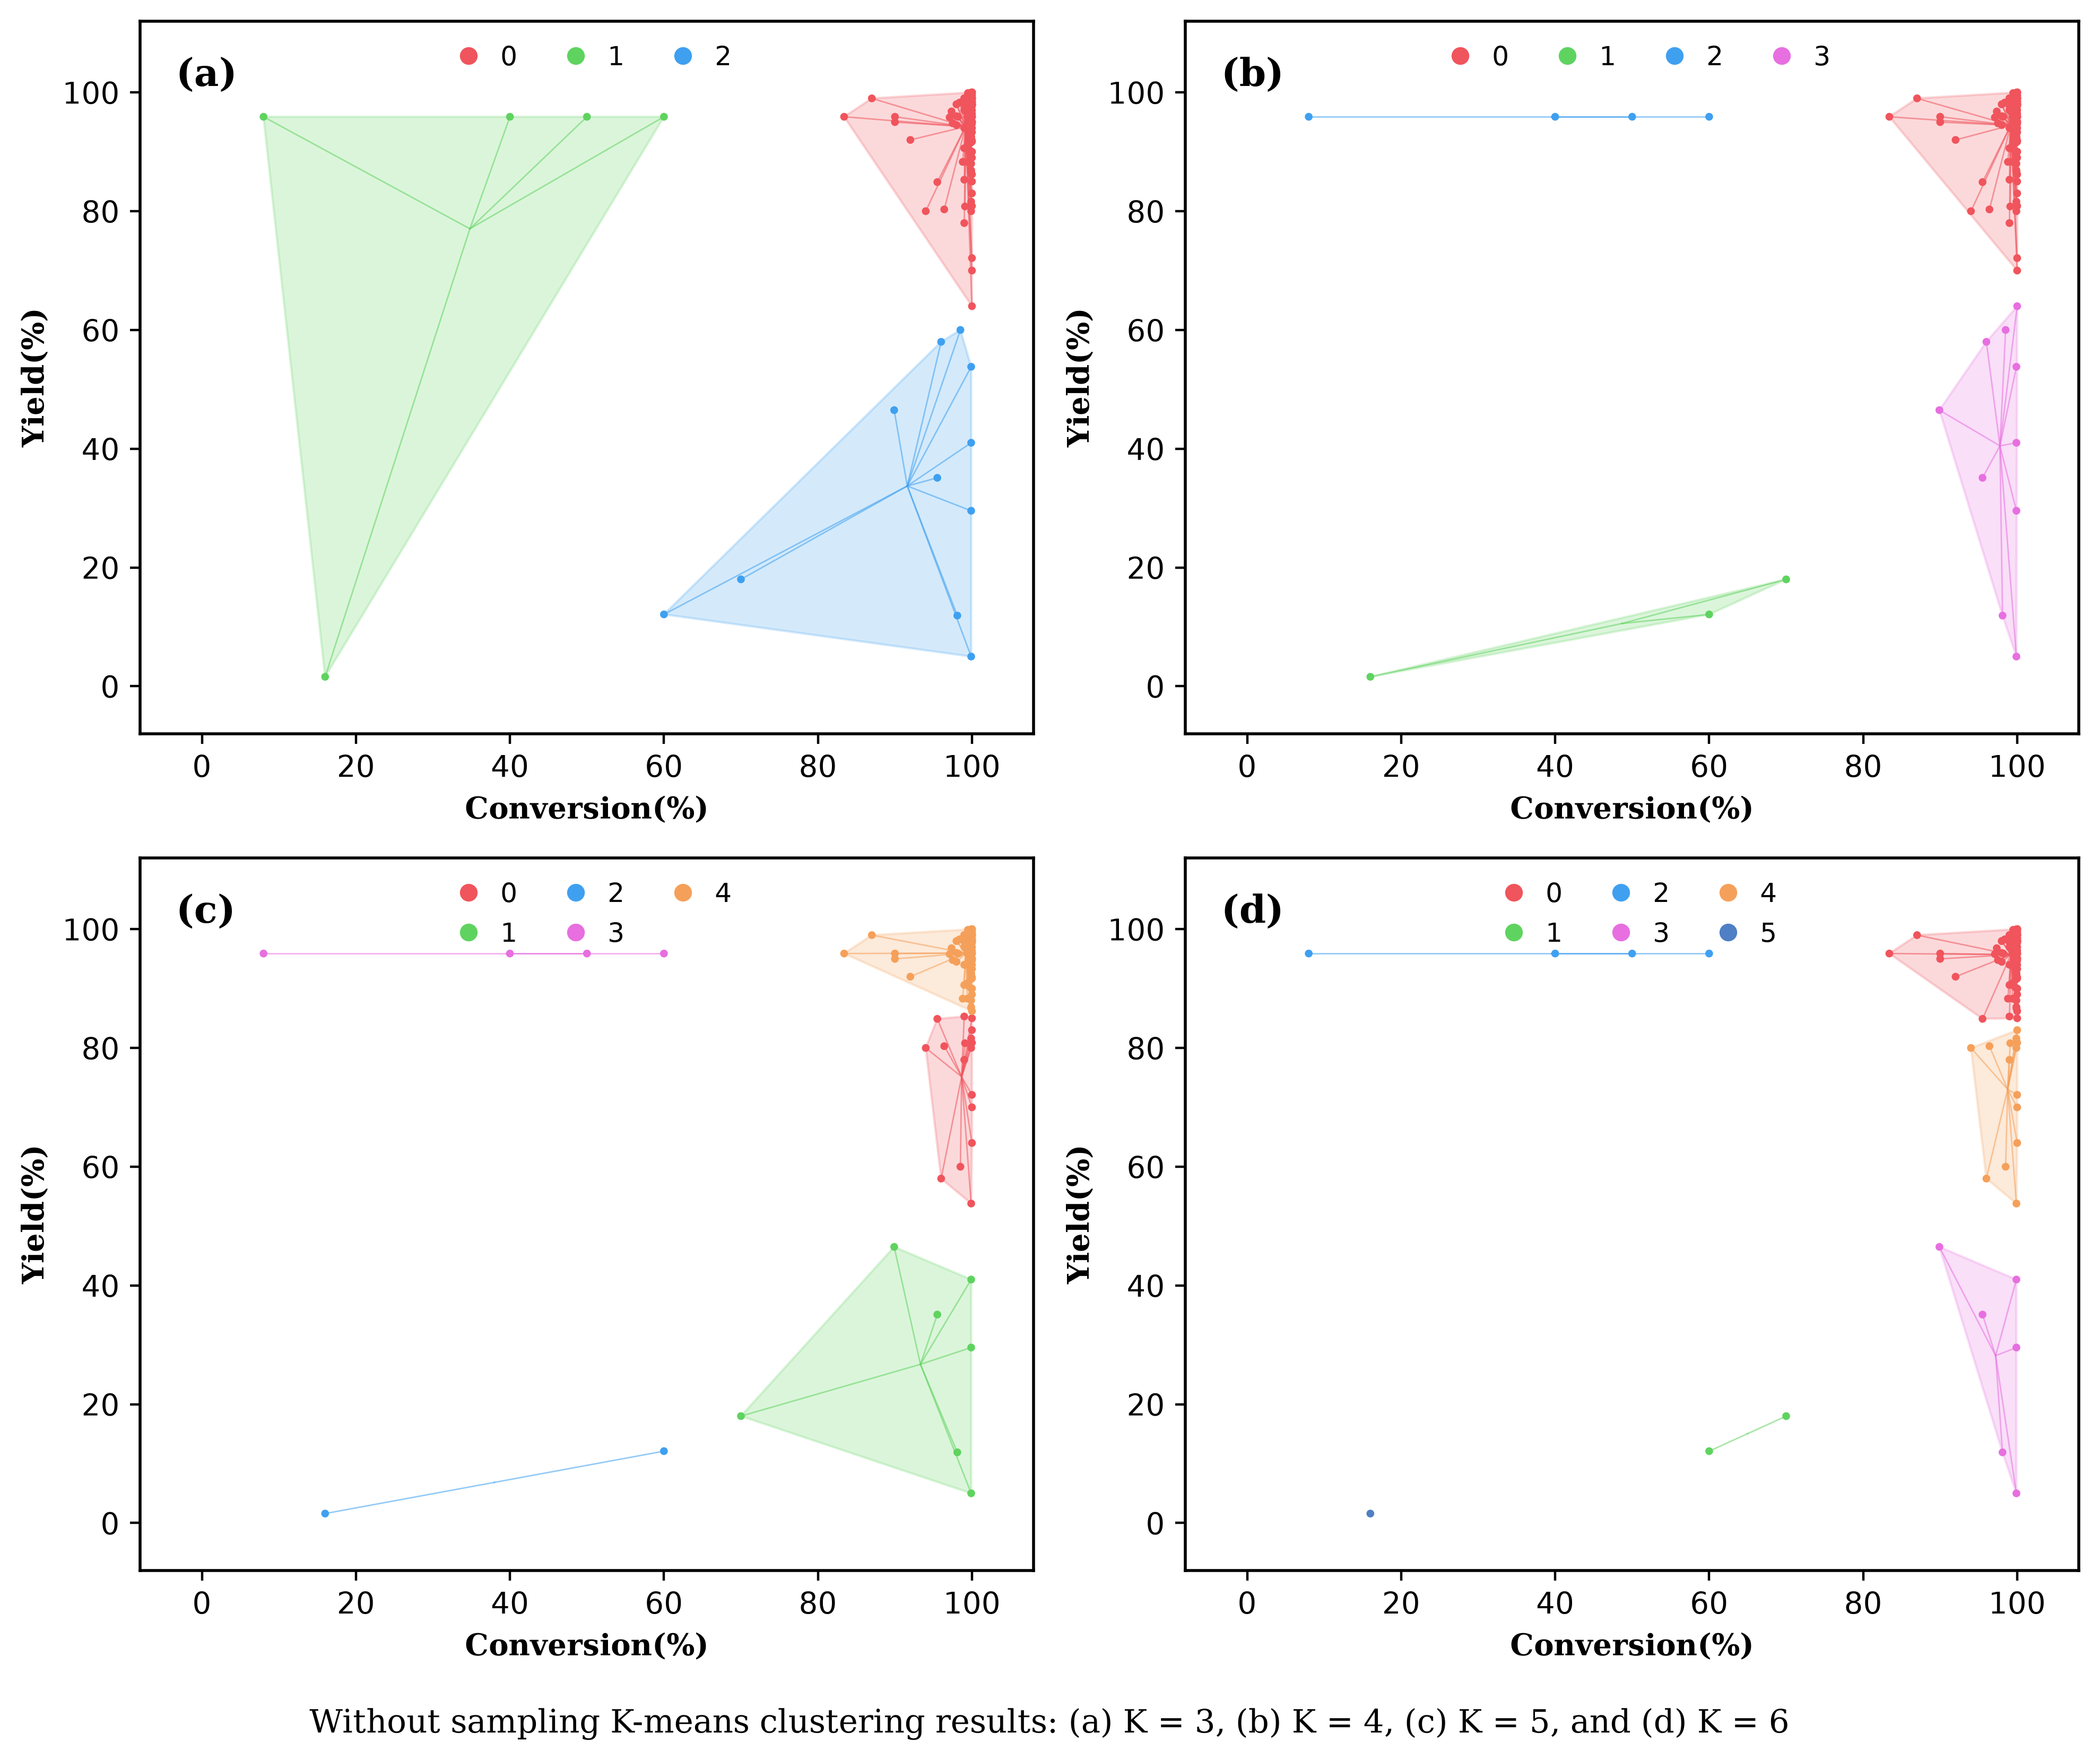
\includegraphics[width=0.78\textwidth,height=0.85\textheight,keepaspectratio]{assets/KMeans_Figure6__HMF_KMeans_Figure6_Style.png}
\caption{K-means clustering of reported conversion and FDCA yield for $K=3$--6.}
\label{fig:kmeans}
\end{figure}
\begin{figure}[!htbp]
\centering
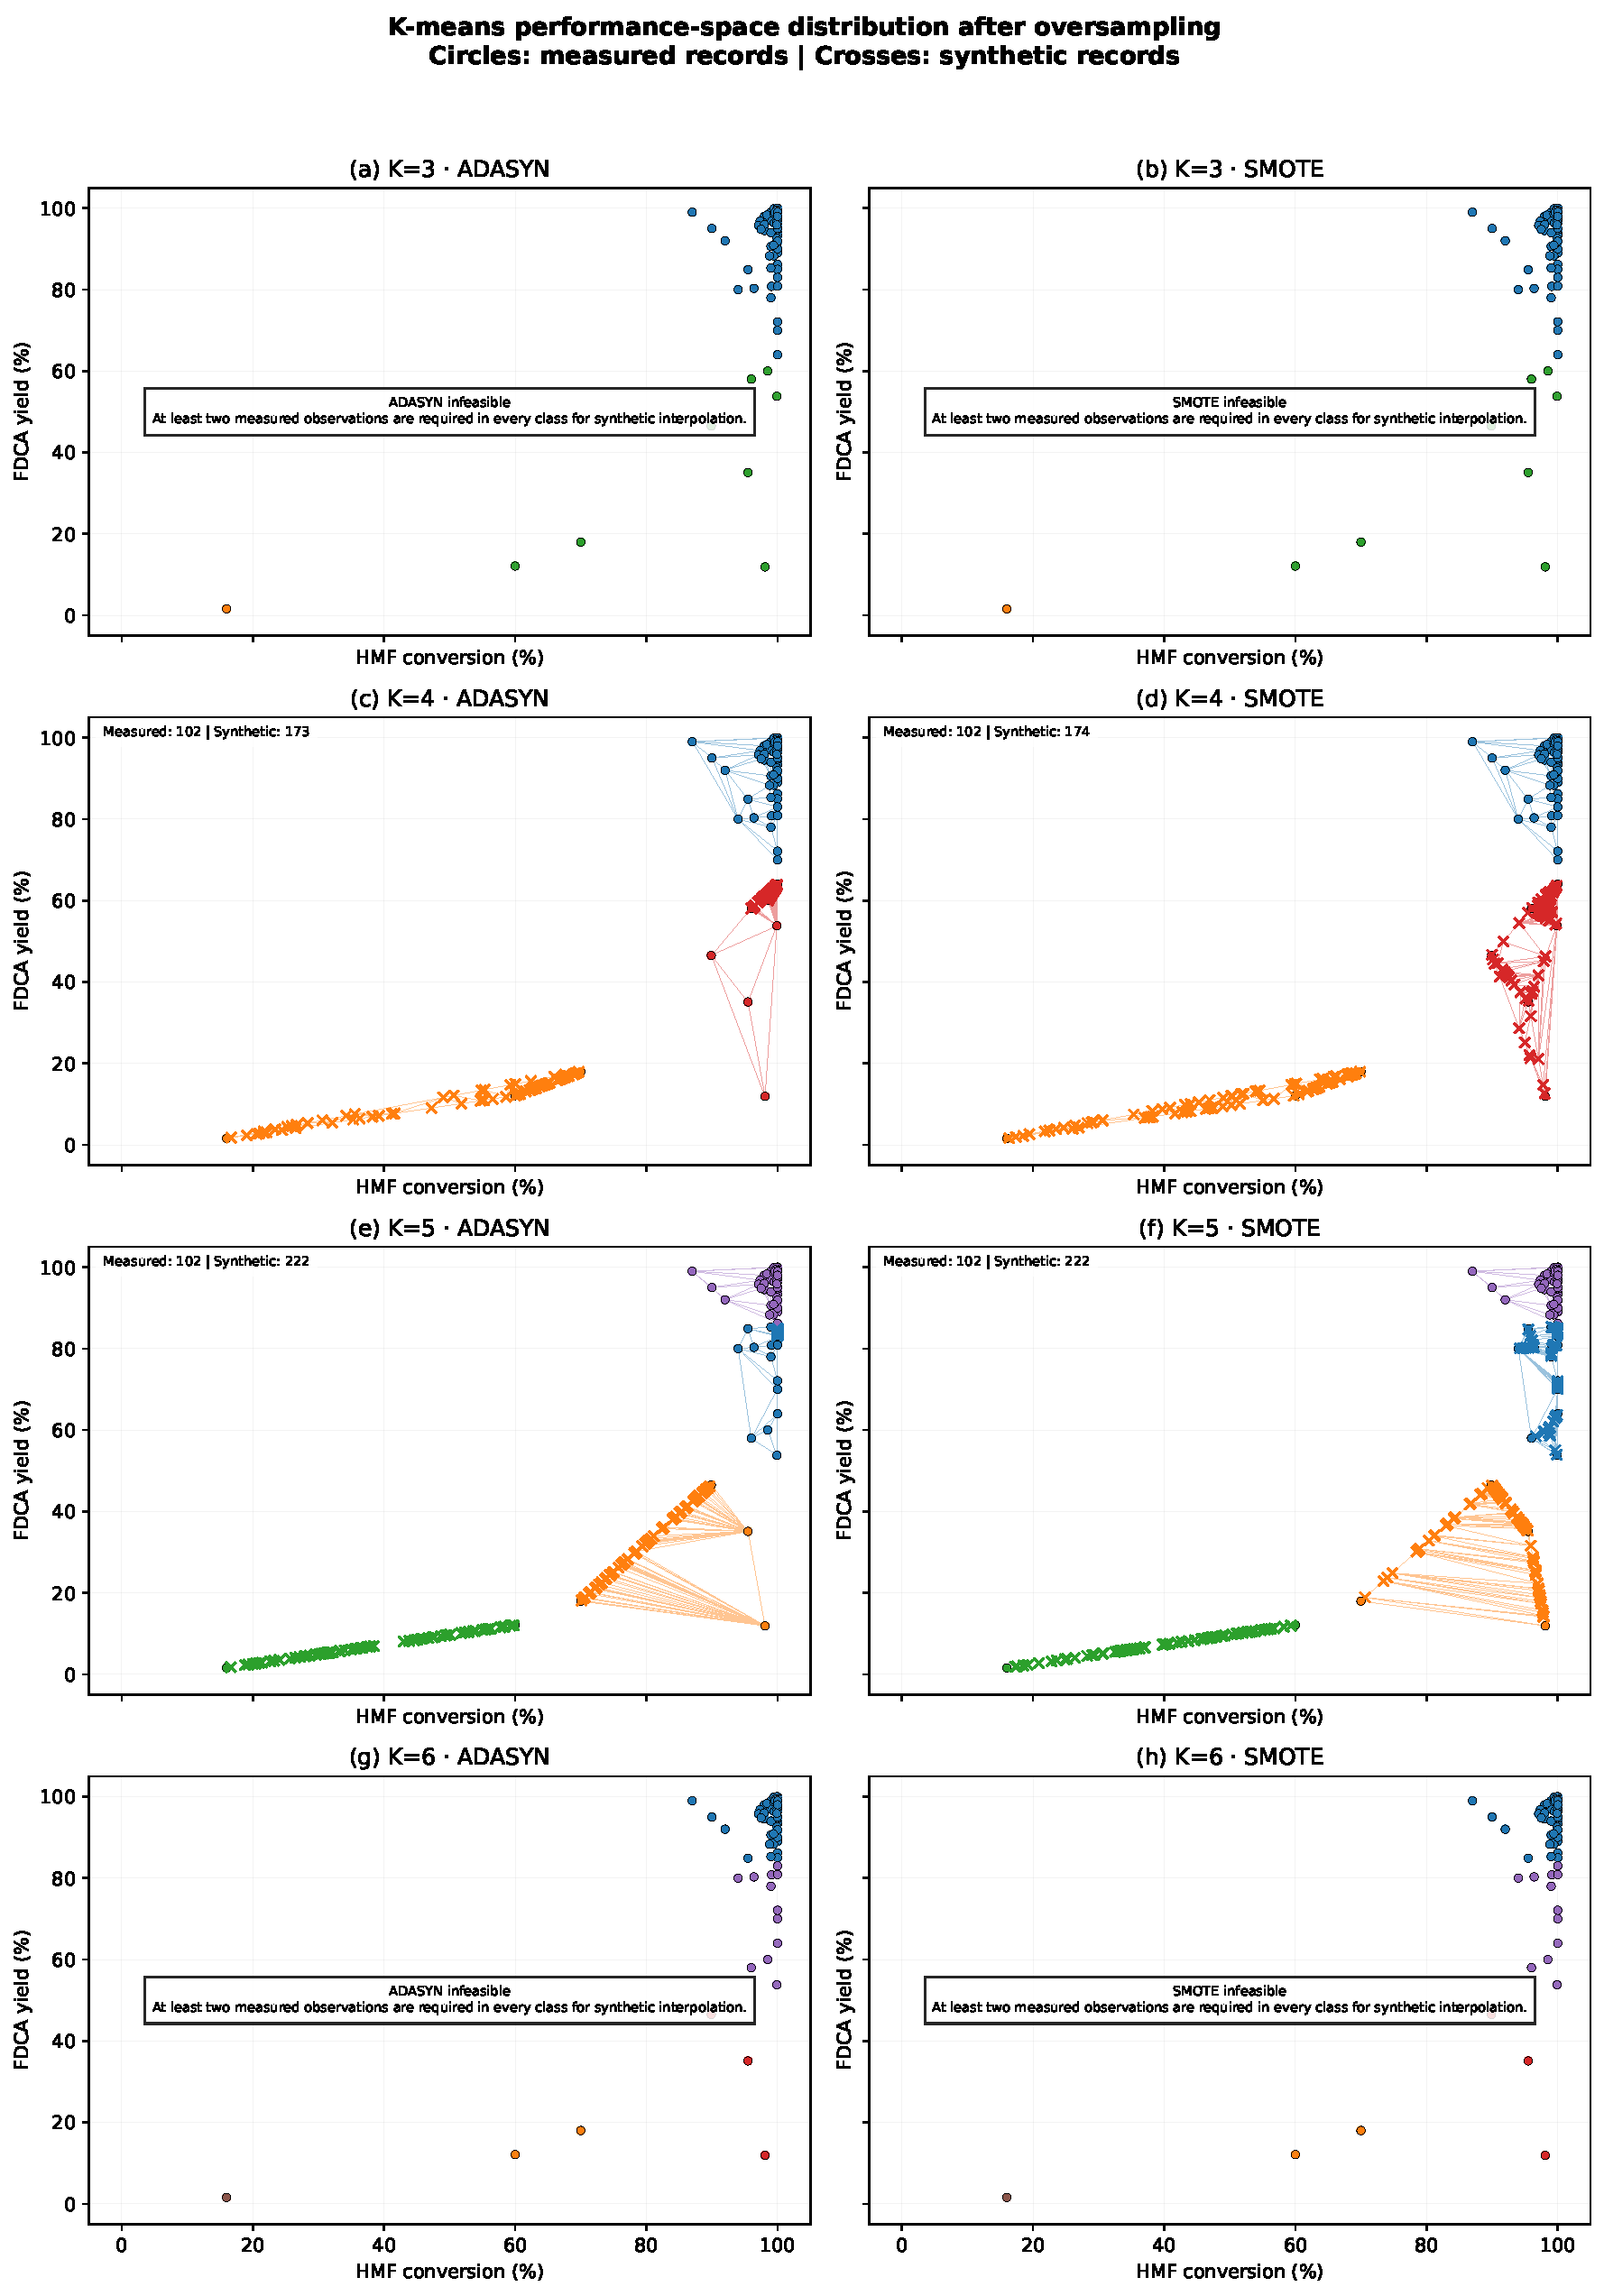
\includegraphics[width=0.85\textwidth,height=0.85\textheight,keepaspectratio]{oversampling_kmeans/KMeans_After_Oversampling_K3_to_K6.pdf}
\caption{ADASYN and SMOTE synthetic records (crosses) in performance space for $K=3$--6, drawn for the 102 records with both outcomes measured. Panels marked infeasible contain a class with fewer than two measured records.}
\label{fig:oversampled}
\end{figure}
\subsection{Classification performance}
Table~\ref{tab:beforeafter} summarises the effect of the revision. For the binary screen (119 records, 89 positive), the best model is the neural network with SMOTE (macro-F1 0.731 $\pm$ 0.033), against 0.480 for a stratified dummy classifier (Table~\ref{tab:binary}, Figure~\ref{fig:binary}). Extra-trees without balancing is statistically indistinguishable (0.720). Every pre-existing family improved on the binary screen, by +0.04 (DT) to +0.22 (NN). For $K=3$ the best model is GB + none (0.626; Table~\ref{tab:k3}). For $K\geq4$, scores stay between 0.2 and 0.45: several classes have fewer than five members, and a single grouped fold frequently contains none of them in training. The within-publication permutation test gives $p=0.47$. Because most descriptors are constant within a paper, shuffling labels inside papers preserves the paper-level signal the model exploits, so this test is conservative here; the dummy comparison and the confidence interval are the more informative checks.

\begin{table}[!htbp]
\centering\small
\caption{Best pooled out-of-fold macro-F1 per classifier family and task (best sampler in parentheses), before (commit \texttt{bdbd2e2}) and after the descriptor, preprocessing, model and evaluation revisions. 95\% CI over 25 repeats. Earlier $K=4$ values were computed on the subset of folds where SMOTE/ADASYN could be fitted and are therefore not comparable (Section~\ref{sec:eval-fix}).}
\label{tab:beforeafter}
\begin{tabular}{llllll}
\toprule
Task & Model & Before & After & 95\% CI & $\Delta$ \\
\midrule
Binary $\geq$90\% & DT & 0.557 (ROS) & 0.600 (ADASYN) & [0.580, 0.619] & +0.042 \\
 & SVM & 0.534 (ADASYN) & 0.695 (ROS) & [0.671, 0.718] & +0.160 \\
 & RF & 0.586 (ROS) & 0.678 (ROS) & [0.659, 0.698] & +0.092 \\
 & NN & 0.507 (ADASYN) & 0.731 (SMOTE) & [0.717, 0.744] & +0.224 \\
 & GB & 0.575 (ROS) & 0.661 (SMOTE) & [0.641, 0.681] & +0.086 \\
 & ET & -- & 0.720 (none) & [0.706, 0.733] & new \\
\midrule
K-means, $K=3$ & DT & 0.410 (ROS) & 0.519 (none) & [0.487, 0.550] & +0.109 \\
 & SVM & 0.298 (ADASYN) & 0.486 (none) & [0.448, 0.524] & +0.187 \\
 & RF & 0.379 (ROS) & 0.481 (ROS) & [0.443, 0.518] & +0.102 \\
 & NN & 0.389 (SMOTE) & 0.535 (ROS) & [0.496, 0.574] & +0.146 \\
 & GB & 0.421 (ROS) & 0.626 (none) & [0.601, 0.650] & +0.205 \\
 & ET & -- & 0.484 (SMOTE) & [0.474, 0.495] & new \\
\midrule
K-means, $K=4$ & DT & 0.360 (SMOTE) & 0.427 (SMOTE) & [0.393, 0.462] & +0.068 \\
 & SVM & 0.458 (SMOTE) & 0.290 (none) & [0.277, 0.302] & -0.168 \\
 & RF & 0.477 (ADASYN) & 0.290 (ROS) & [0.281, 0.300] & -0.187 \\
 & NN & 0.248 (ADASYN) & 0.318 (SMOTE) & [0.300, 0.337] & +0.071 \\
 & GB & 0.437 (SMOTE) & 0.314 (SMOTE) & [0.306, 0.323] & -0.123 \\
 & ET & -- & 0.325 (SMOTE) & [0.318, 0.331] & new \\
\midrule
K-means, $K=5$ & DT & 0.232 (ROS) & 0.220 (ROS) & [0.211, 0.229] & -0.012 \\
 & SVM & 0.255 (none) & 0.302 (ROS) & [0.296, 0.307] & +0.047 \\
 & RF & 0.272 (ROS) & 0.286 (ROS) & [0.279, 0.293] & +0.014 \\
 & NN & 0.237 (ROS) & 0.321 (ROS) & [0.307, 0.335] & +0.084 \\
 & GB & 0.265 (ROS) & 0.278 (none) & [0.268, 0.289] & +0.014 \\
 & ET & -- & 0.298 (none) & [0.286, 0.310] & new \\
\midrule
K-means, $K=6$ & DT & 0.215 (ROS) & 0.225 (none) & [0.212, 0.238] & +0.010 \\
 & SVM & 0.215 (none) & 0.245 (ROS) & [0.238, 0.253] & +0.030 \\
 & RF & 0.215 (ROS) & 0.250 (ROS) & [0.246, 0.255] & +0.035 \\
 & NN & 0.198 (ROS) & 0.283 (ROS) & [0.268, 0.299] & +0.085 \\
 & GB & 0.207 (none) & 0.231 (ROS) & [0.225, 0.237] & +0.024 \\
 & ET & -- & 0.254 (ROS) & [0.247, 0.261] & new \\
\bottomrule
\end{tabular}
\end{table}
\begin{table}[!htbp]
\centering\small
\caption{Binary $\geq$90\% screen: pooled out-of-fold macro-F1 (mean $\pm$ SD over 25 repeats) for every model and sampler.}
\label{tab:binary}
\begin{tabular}{lcccc}
\toprule
Model & None & ROS & SMOTE & ADASYN \\
\midrule
DT & 0.593 $\pm$ 0.031 & 0.593 $\pm$ 0.040 & 0.598 $\pm$ 0.042 & 0.600 $\pm$ 0.047 \\
SVM & 0.681 $\pm$ 0.032 & 0.695 $\pm$ 0.056 & 0.630 $\pm$ 0.043 & 0.637 $\pm$ 0.026 \\
RF & 0.658 $\pm$ 0.042 & 0.678 $\pm$ 0.047 & 0.640 $\pm$ 0.036 & 0.630 $\pm$ 0.027 \\
NN & 0.718 $\pm$ 0.038 & 0.718 $\pm$ 0.037 & \textbf{0.731 $\pm$ 0.033} & 0.721 $\pm$ 0.035 \\
GB & 0.568 $\pm$ 0.033 & 0.631 $\pm$ 0.045 & 0.661 $\pm$ 0.048 & 0.645 $\pm$ 0.047 \\
ET & 0.720 $\pm$ 0.032 & 0.696 $\pm$ 0.041 & 0.716 $\pm$ 0.038 & 0.713 $\pm$ 0.030 \\
\bottomrule
\end{tabular}
\end{table}
\begin{table}[!htbp]
\centering\small
\caption{K-means $K=3$: pooled out-of-fold macro-F1 (mean $\pm$ SD over 25 repeats).}
\label{tab:k3}
\begin{tabular}{lcccc}
\toprule
Model & None & ROS & SMOTE & ADASYN \\
\midrule
DT & 0.519 $\pm$ 0.076 & 0.512 $\pm$ 0.079 & 0.450 $\pm$ 0.056 & 0.454 $\pm$ 0.065 \\
SVM & 0.486 $\pm$ 0.093 & 0.403 $\pm$ 0.102 & 0.436 $\pm$ 0.099 & 0.422 $\pm$ 0.085 \\
RF & 0.328 $\pm$ 0.024 & 0.481 $\pm$ 0.091 & 0.358 $\pm$ 0.037 & 0.360 $\pm$ 0.040 \\
NN & 0.438 $\pm$ 0.073 & 0.535 $\pm$ 0.095 & 0.515 $\pm$ 0.084 & 0.520 $\pm$ 0.084 \\
GB & \textbf{0.626 $\pm$ 0.060} & 0.591 $\pm$ 0.043 & 0.604 $\pm$ 0.081 & 0.603 $\pm$ 0.097 \\
ET & 0.457 $\pm$ 0.047 & 0.444 $\pm$ 0.041 & 0.484 $\pm$ 0.026 & 0.478 $\pm$ 0.027 \\
\bottomrule
\end{tabular}
\end{table}
\begin{figure}[!htbp]
\centering
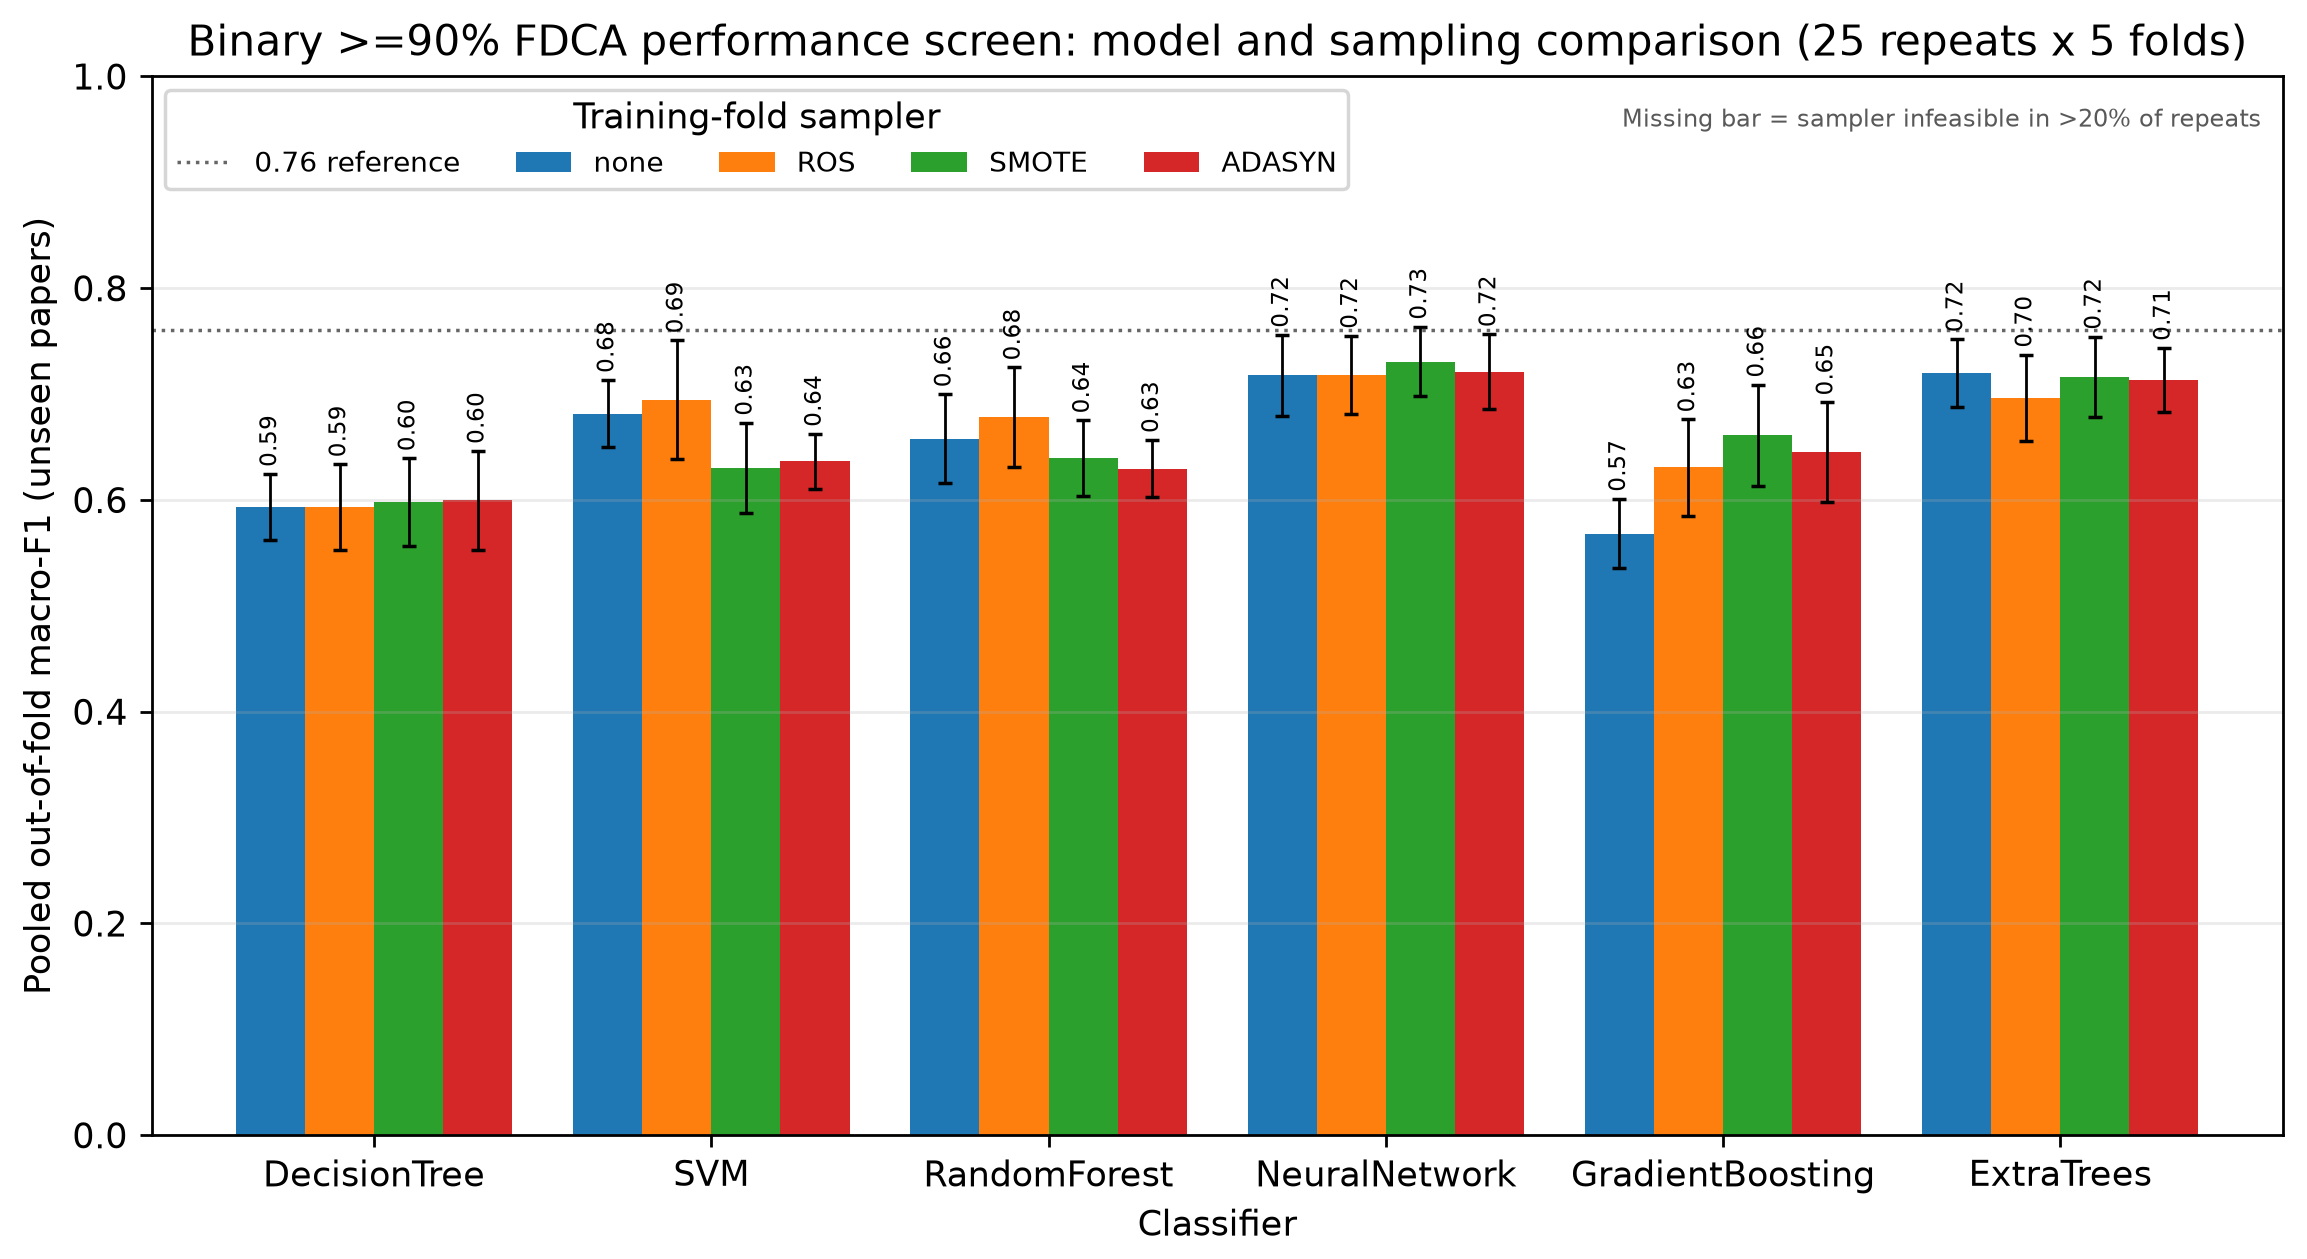
\includegraphics[width=\textwidth,height=0.85\textheight,keepaspectratio]{assets/classification__model_sampler_binary90.png}
\caption{Binary $\geq$90\% screen: pooled out-of-fold macro-F1 by classifier and training-fold sampler (error bars: SD over 25 repeats; dotted line: 0.76).}
\label{fig:binary}
\end{figure}
\begin{figure}[!htbp]
\centering
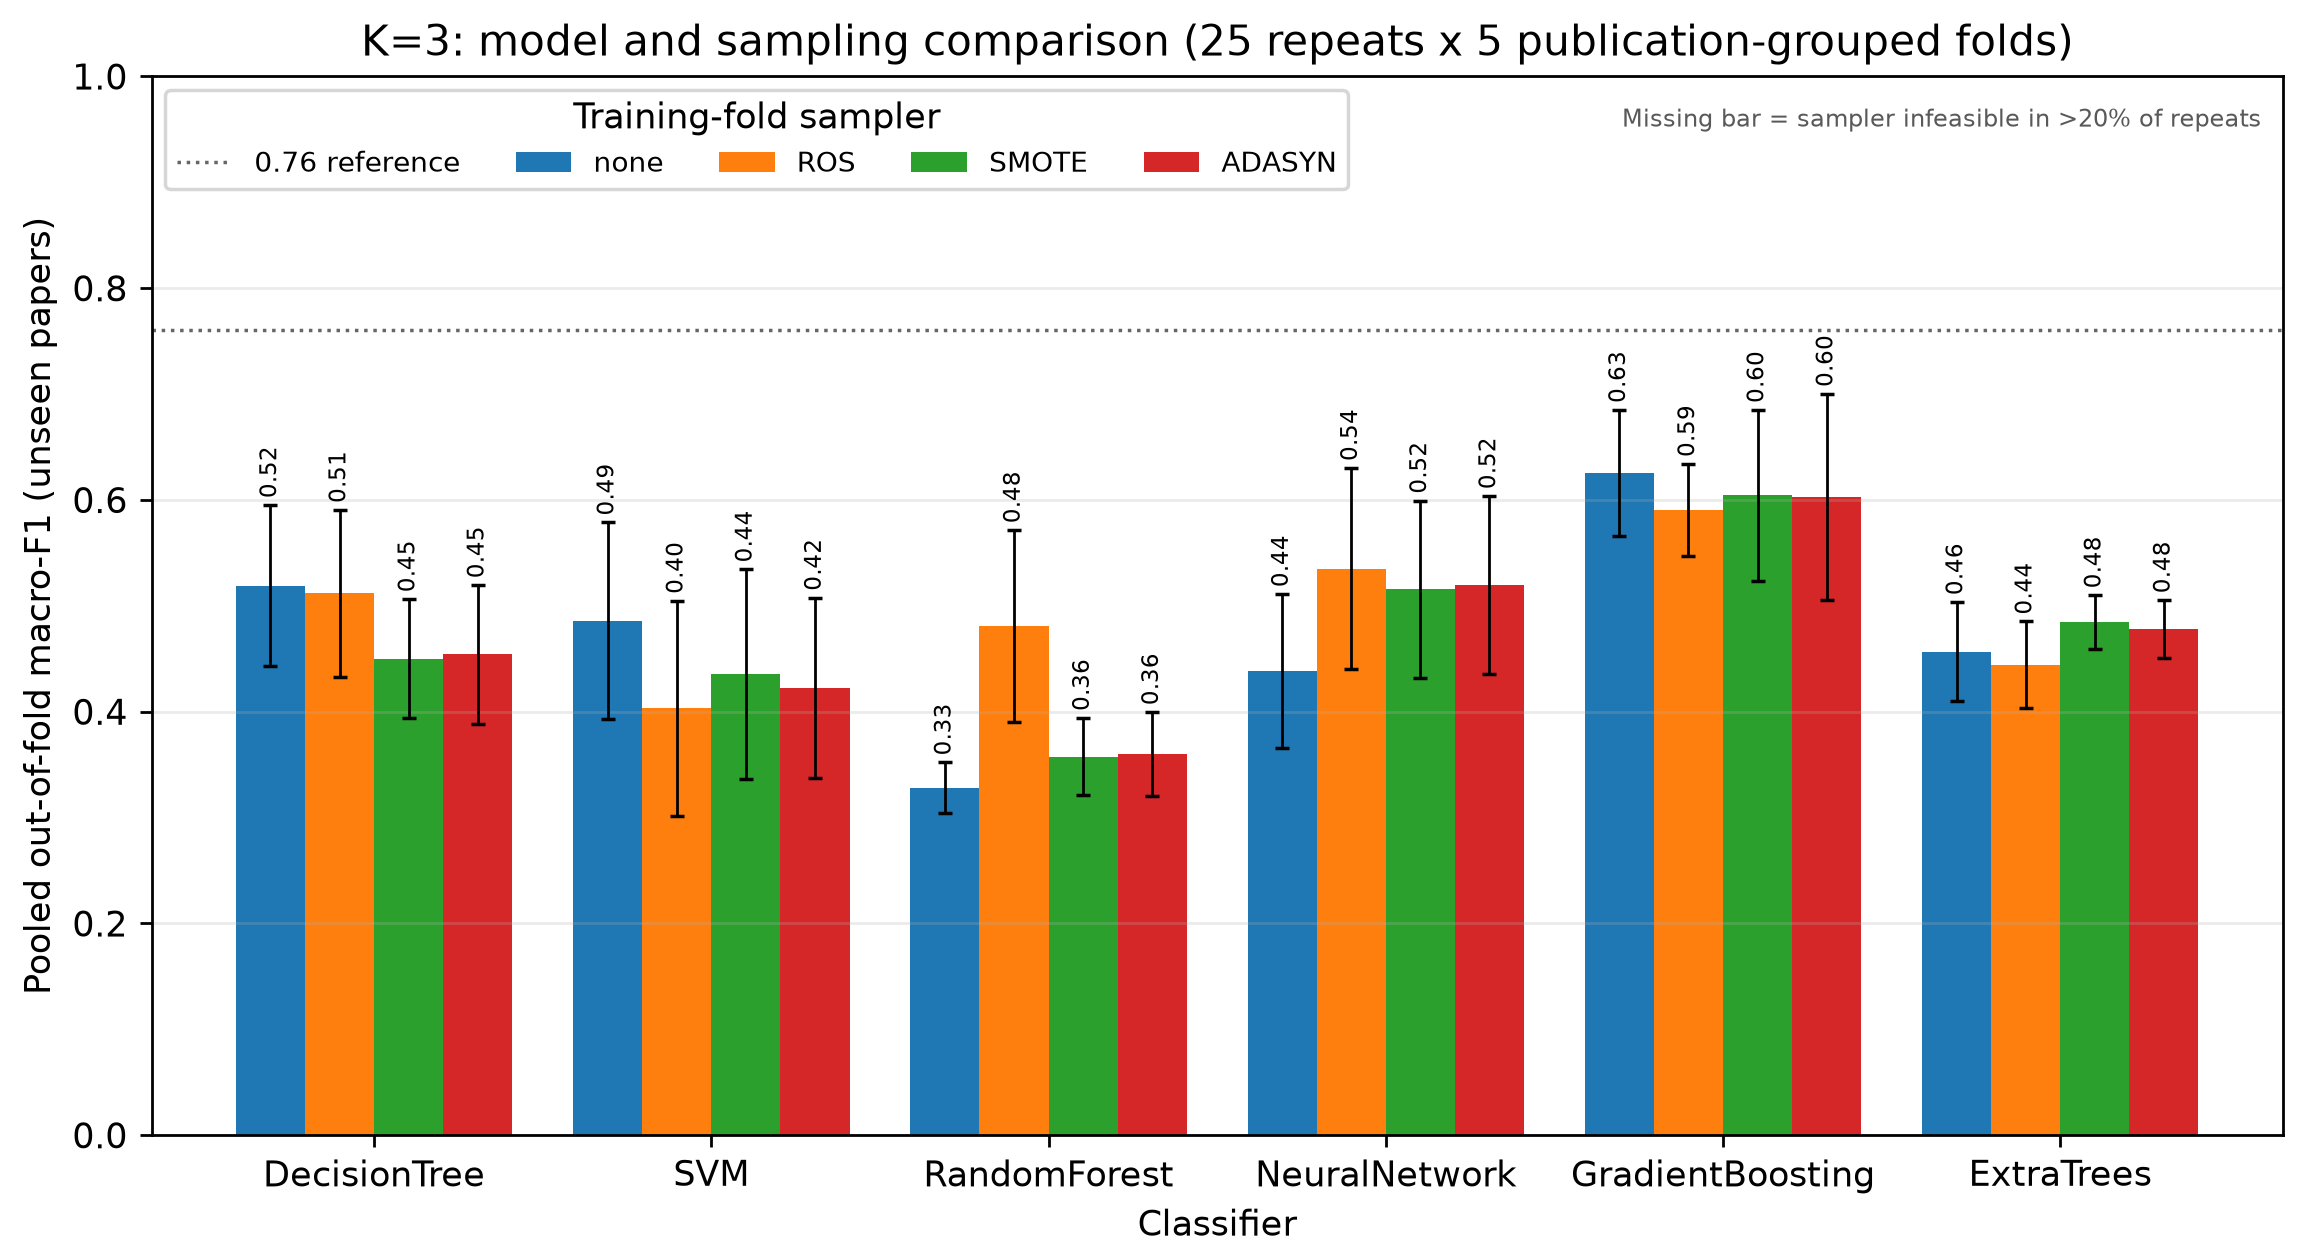
\includegraphics[width=\textwidth,height=0.85\textheight,keepaspectratio]{assets/classification__model_sampler_K3.png}
\caption{K-means $K=3$: pooled out-of-fold macro-F1 by classifier and sampler.}
\label{fig:k3}
\end{figure}
\begin{figure}[!htbp]
\centering
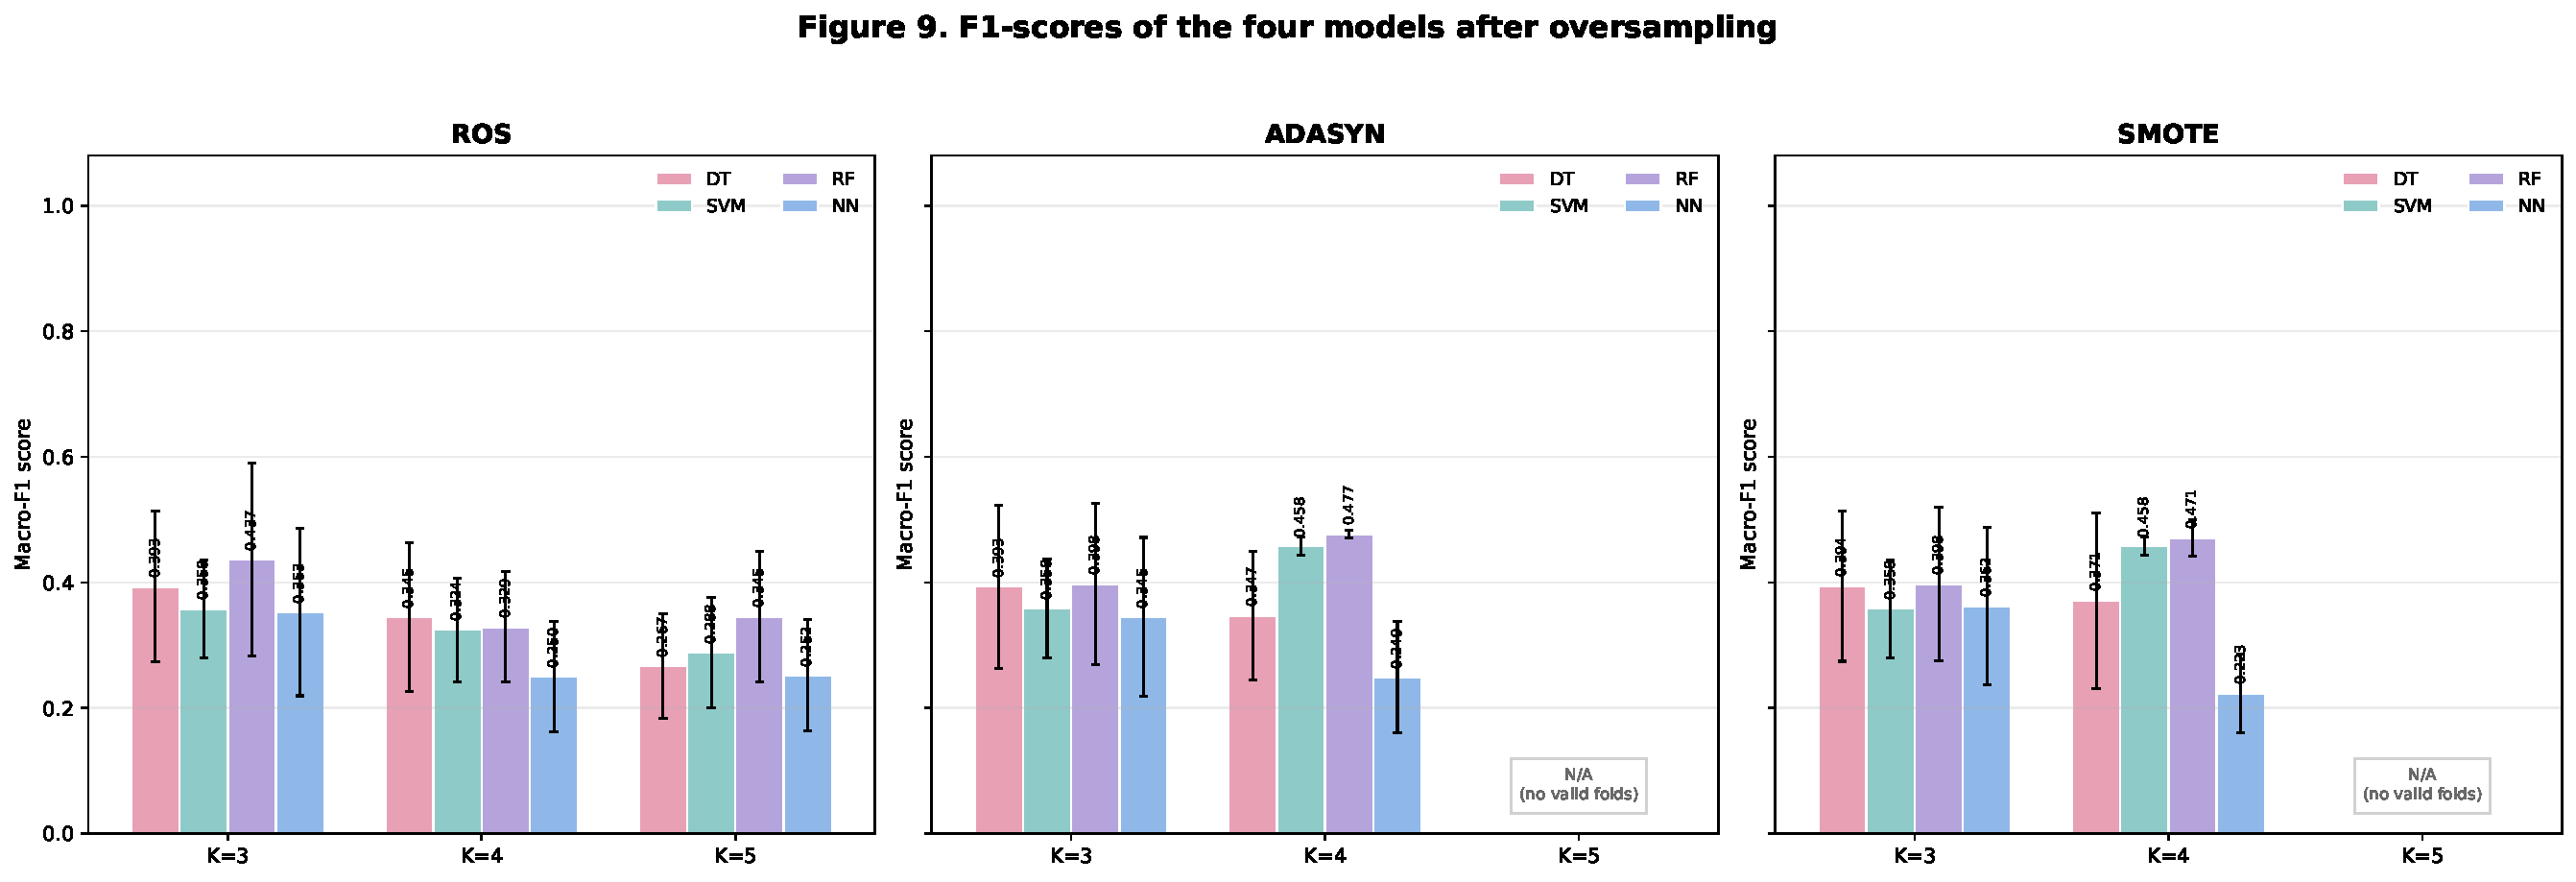
\includegraphics[width=\textwidth,height=0.85\textheight,keepaspectratio]{paper_style/Figure_9_Oversampling_F1.pdf}
\caption{Fold-averaged macro-F1 of DT, SVM, RF and NN after ROS, ADASYN and SMOTE for $K=3$--5 (reference-paper layout). Fold averages are computed over feasible folds only and differ from the pooled scores in Table~\ref{tab:beforeafter}.}
\label{fig:fig9}
\end{figure}
\begin{figure}[!htbp]
\centering
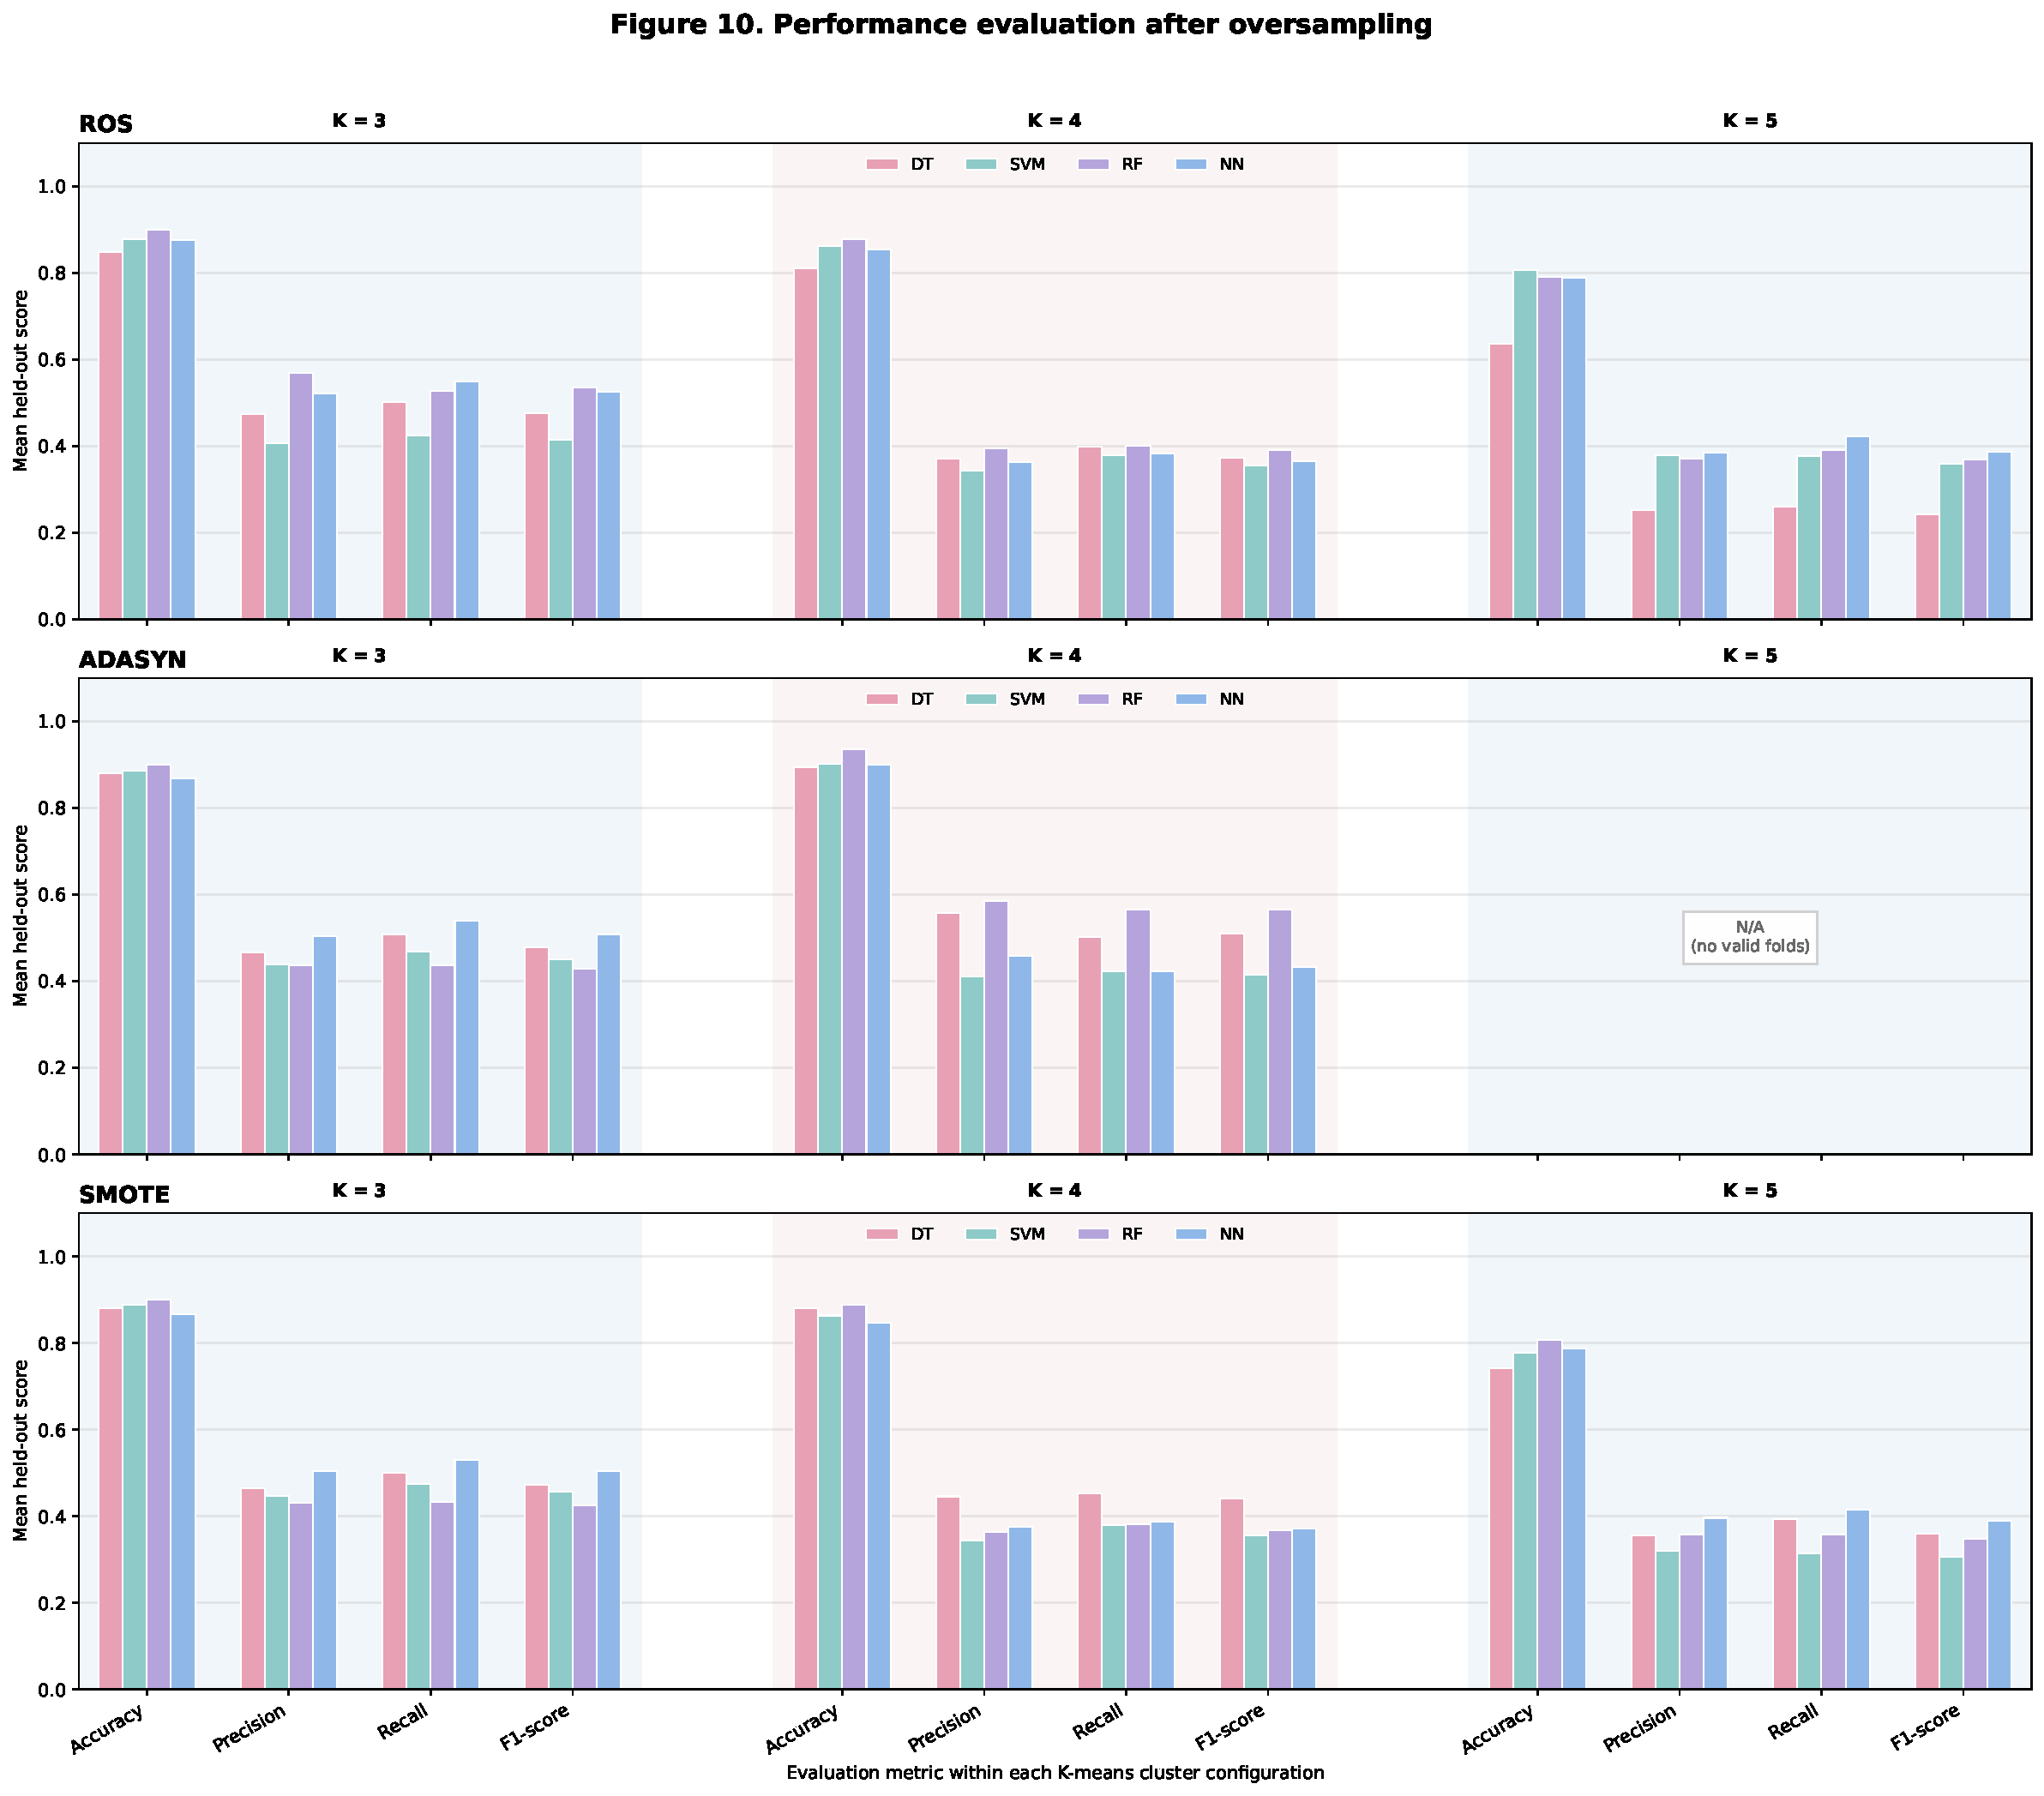
\includegraphics[width=\textwidth,height=0.85\textheight,keepaspectratio]{paper_style/Figure_10_Performance_Metrics.pdf}
\caption{Accuracy, precision, recall and F1 after oversampling.}
\label{fig:fig10}
\end{figure}
\subsection{Learning curves}
Training macro-F1 stays well above validation macro-F1 for every model and $K$ (Table~\ref{tab:learning}, Figure~\ref{fig:learning}), indicating variance-limited models. At $K=3$ the SVM validation curve is still rising at the largest training size and the other families fluctuate without a clear plateau, so additional publications are the most direct route to higher scores; for $K\geq4$ the curves are flat because the minority clusters do not grow with more records.
\begin{table}[!htbp]
\centering\small
\caption{Learning-curve end points (full training fraction, publication-grouped 80/20 holdouts, 10 repeats).}
\label{tab:learning}
\begin{tabular}{rlrrr}
\toprule
$K$ & Model & Train macro-F1 & Validation macro-F1 & Gap \\
\midrule
3 & DT & 0.920 & 0.481 & 0.438 \\
3 & NN & 0.959 & 0.537 & 0.421 \\
3 & RF & 0.939 & 0.470 & 0.469 \\
3 & SVM & 0.834 & 0.729 & 0.105 \\
4 & DT & 0.556 & 0.286 & 0.269 \\
4 & NN & 0.969 & 0.299 & 0.670 \\
4 & RF & 0.959 & 0.228 & 0.731 \\
4 & SVM & 0.909 & 0.223 & 0.685 \\
5 & DT & 0.740 & 0.209 & 0.532 \\
5 & NN & 0.774 & 0.315 & 0.458 \\
5 & RF & 0.874 & 0.231 & 0.642 \\
5 & SVM & 0.734 & 0.250 & 0.483 \\
\bottomrule
\end{tabular}
\end{table}
\begin{figure}[!htbp]
\centering
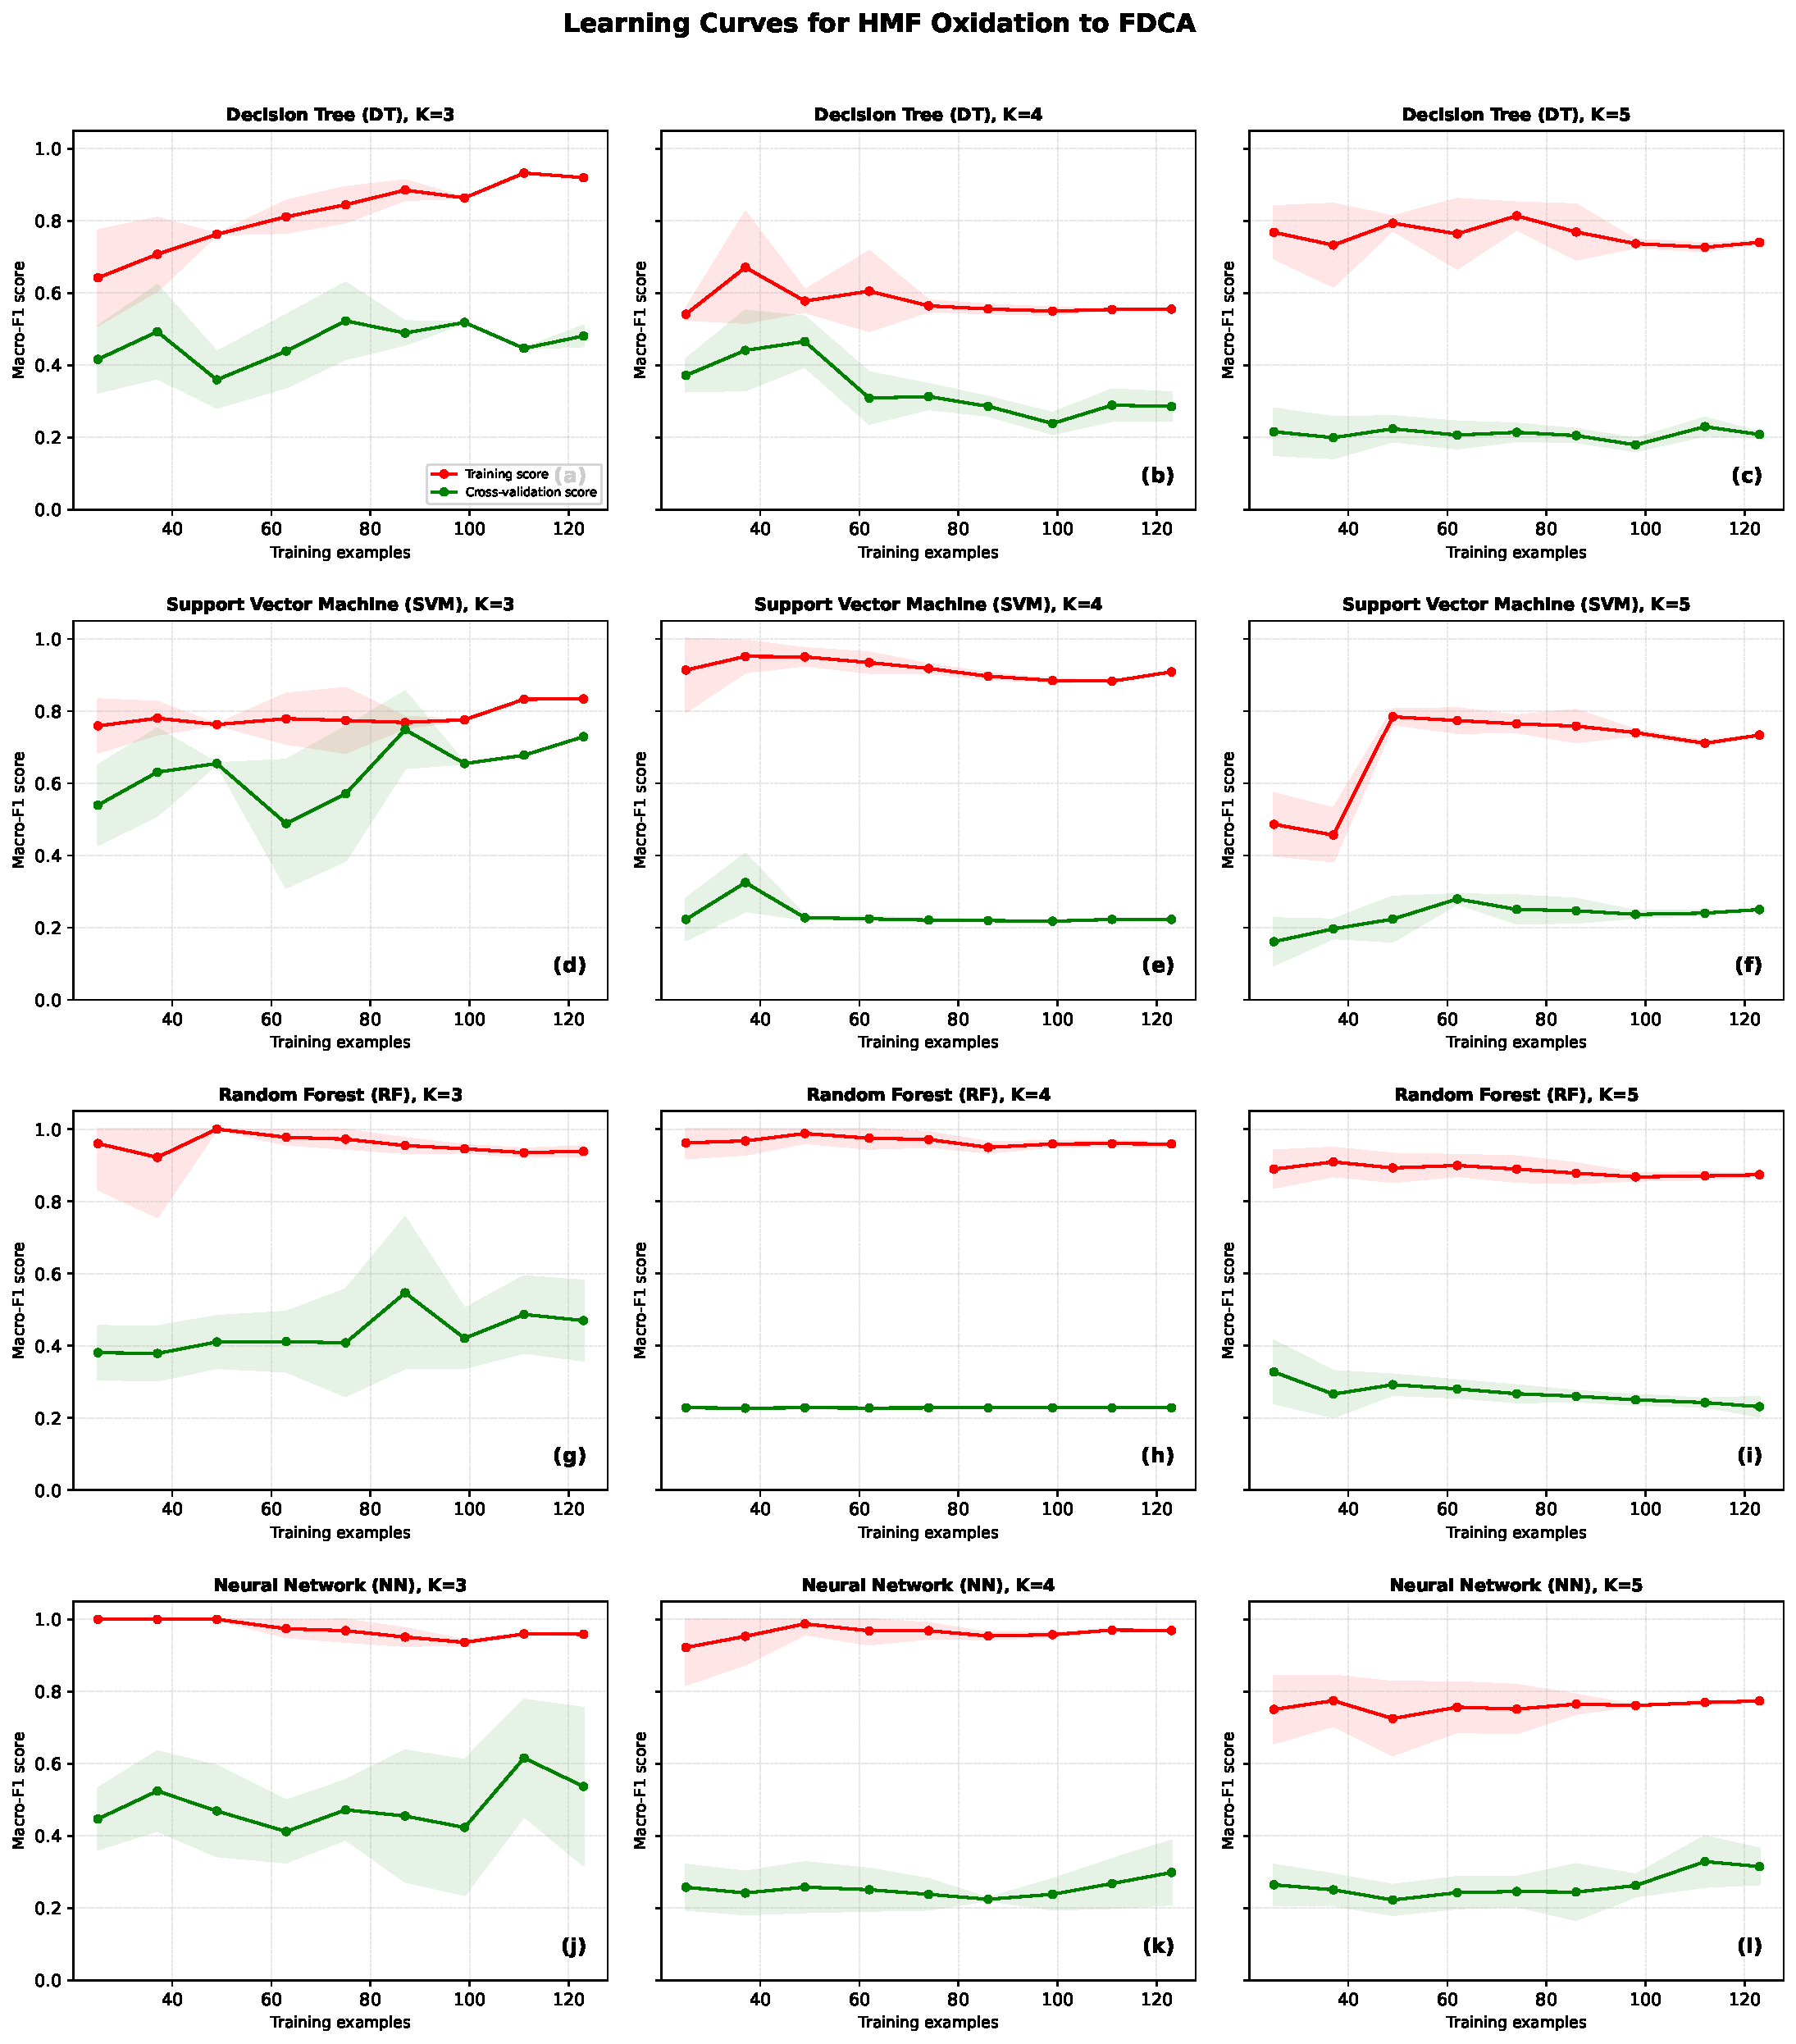
\includegraphics[width=\textwidth,height=0.85\textheight,keepaspectratio]{learning_curves/HMF_Learning_Curves_Figure.pdf}
\caption{Learning curves (macro-F1) for DT, SVM, RF and NN at $K=3$, 4 and 5 with publication-grouped holdouts; shading shows $\pm$1 SD.}
\label{fig:learning}
\end{figure}
\begin{figure}[!htbp]
\centering
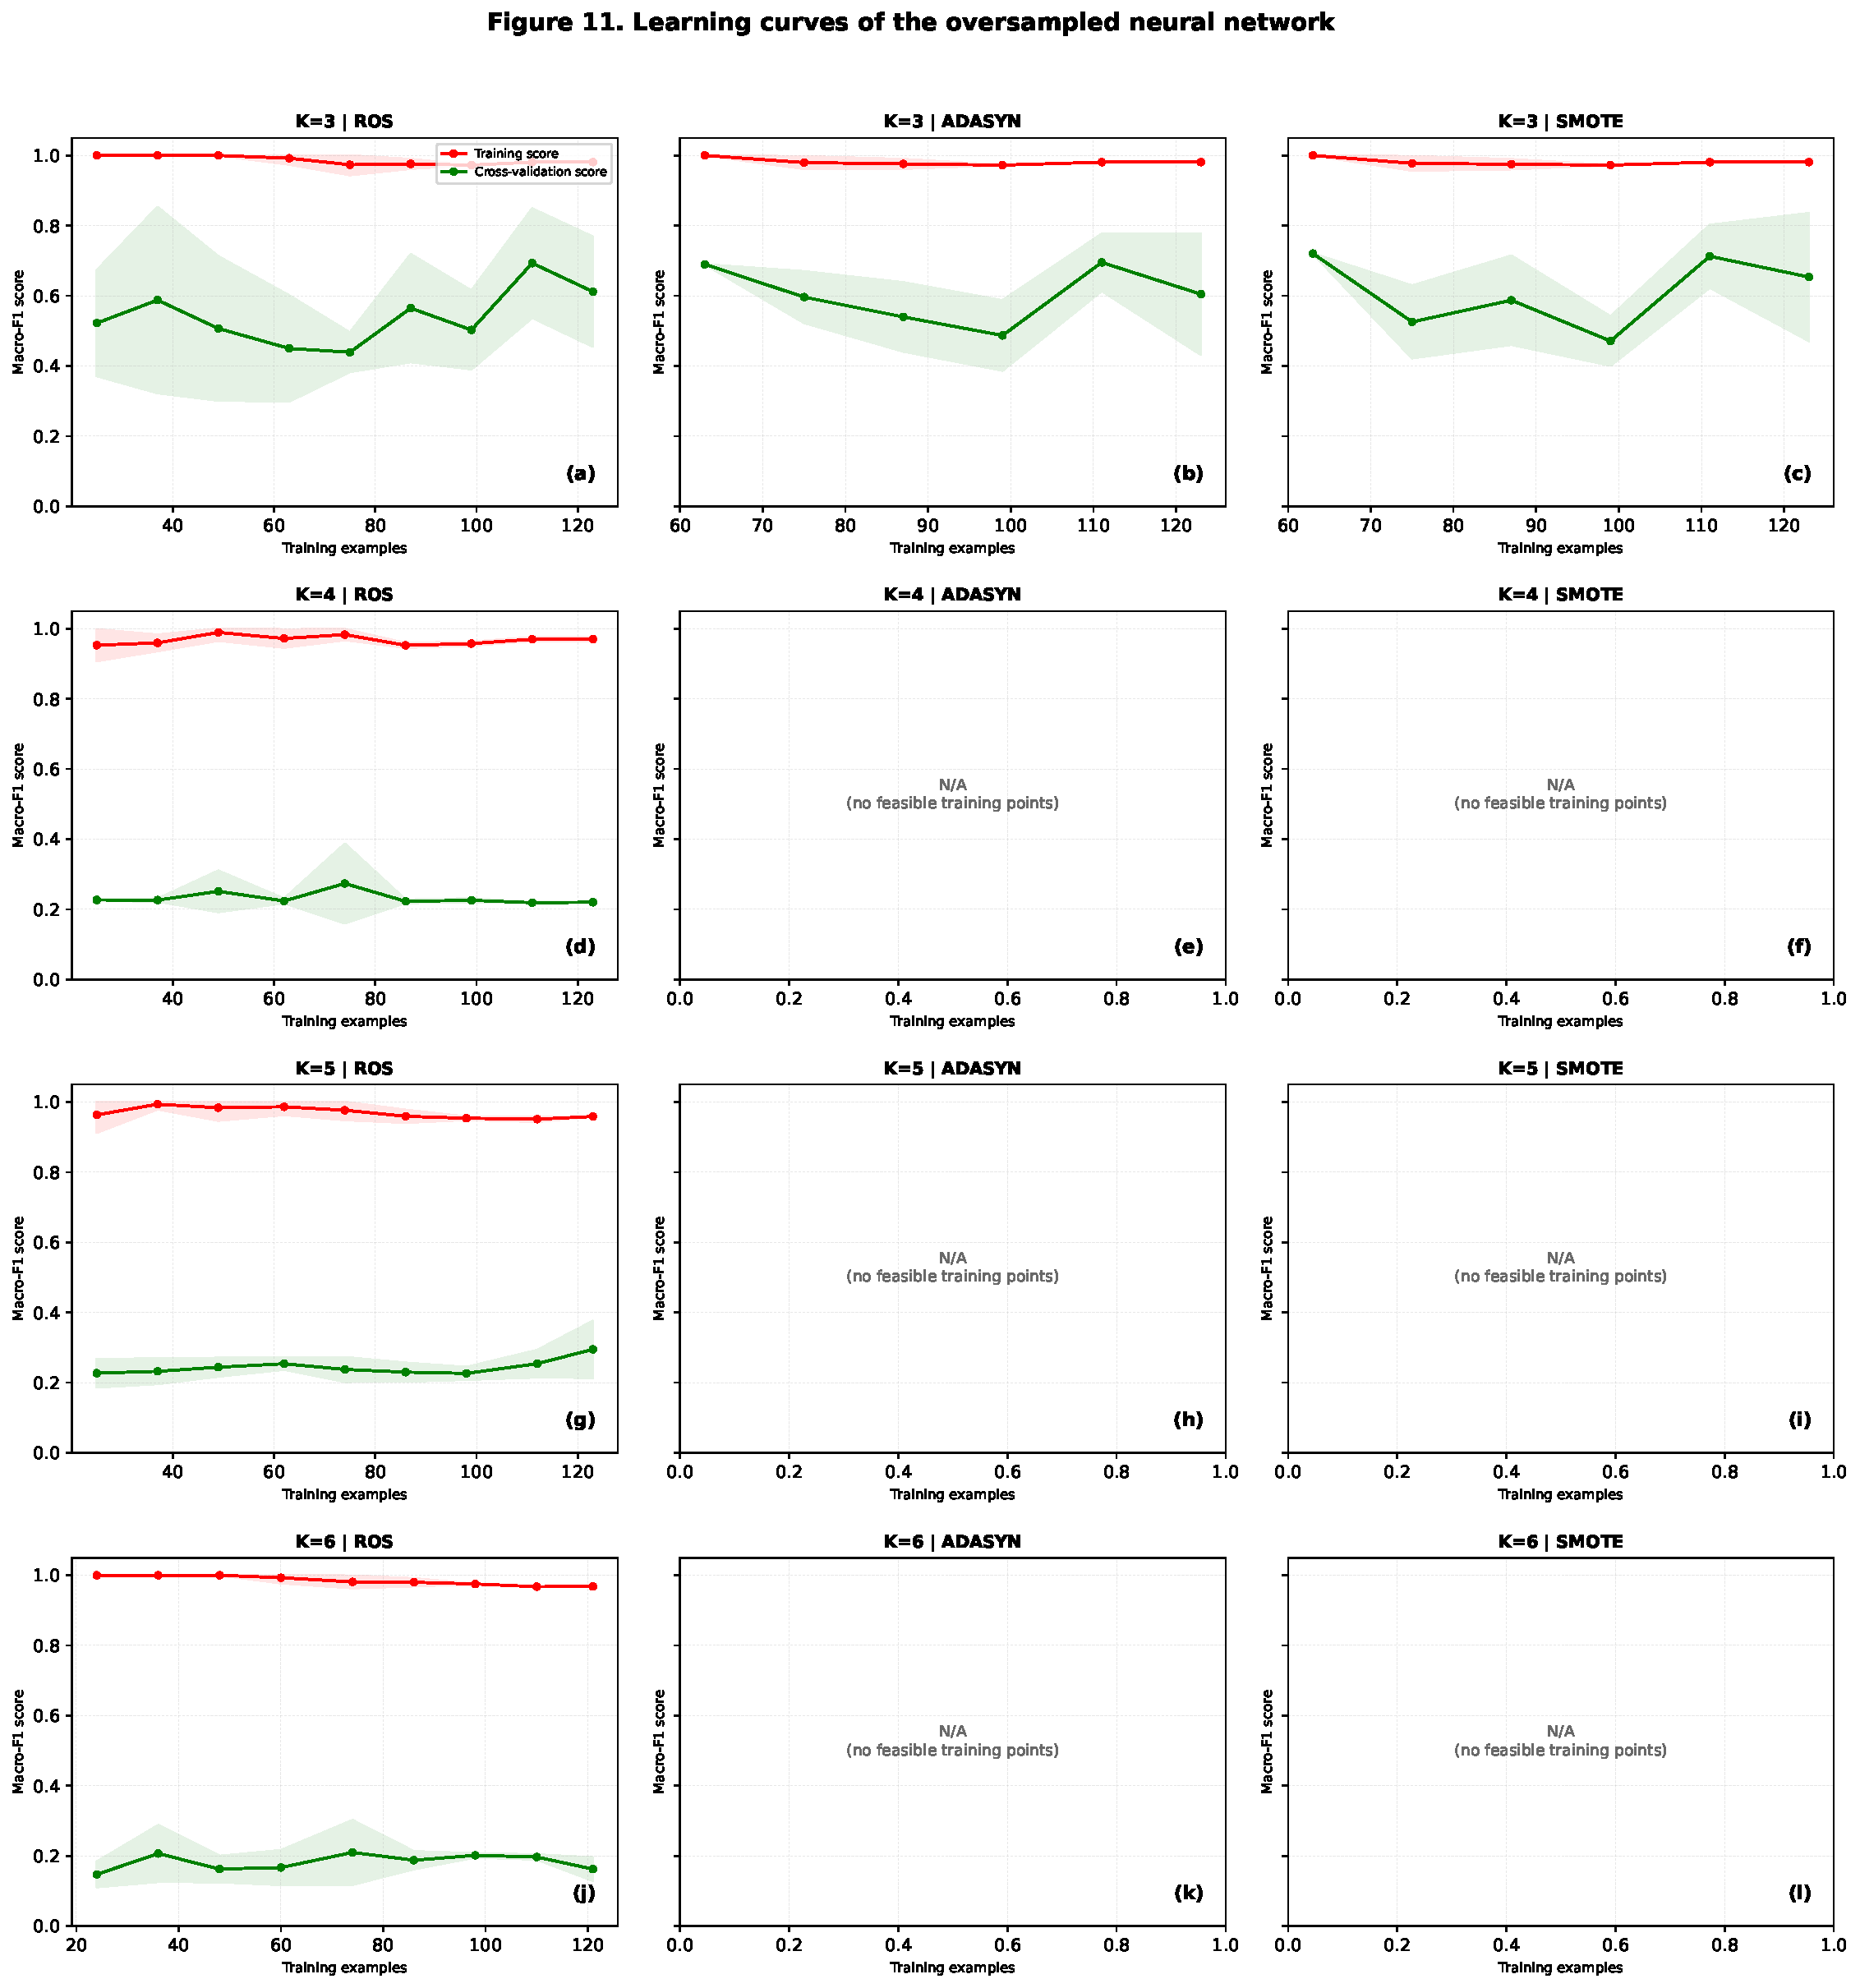
\includegraphics[width=\textwidth,height=0.85\textheight,keepaspectratio]{learning_curves/Figure_11_Oversampled_NN_Learning_Curves_ROS_ADASYN_SMOTE.pdf}
\caption{Neural-network learning curves with ROS, ADASYN and SMOTE applied to training folds only.}
\label{fig:fig11}
\end{figure}
\subsection{Model interpretation}
Table~\ref{tab:shap} and Figures~\ref{fig:shapsel}--\ref{fig:fig13} list the descriptors with the largest SHAP contributions. Support type (conductive glass versus foam), copper and iron content, oxyhydroxide/hydroxide phases, counter-electrode material, potential and the temperature-not-reported indicator recur across models. These rankings describe what the models use to separate the literature records; they partly encode publication style and are not evidence of causal catalyst effects.
\begin{table*}[!htbp]
\centering\scriptsize
\caption{Top-ranked descriptors by mean absolute SHAP value on held-out publications. Values are associational, not causal; \texttt{missingindicator\_*} columns flag unreported conditions.}
\label{tab:shap}
\resizebox{\textwidth}{!}{%
\begin{tabular}{lrlrlr}
\toprule
\multicolumn{2}{c}{Binary screen (NN + SMOTE)} & \multicolumn{2}{c}{$K=3$ (GB + none)} & \multicolumn{2}{c}{$K=5$ (NN + ROS)} \\
\cmidrule(lr){1-2}\cmidrule(lr){3-4}\cmidrule(lr){5-6}
\texttt{Catalyst\_Conductive\_Glass} & 0.104 & \texttt{Catalyst\_Conductive\_Glass} & 0.096 & \texttt{Catalyst\_Pd} & 0.019 \\
\texttt{Catalyst\_Oxyhydroxide} & 0.053 & \texttt{Potential\_vs\_RHE\_V} & 0.023 & \texttt{Catalyst\_Conductive\_Glass} & 0.013 \\
\texttt{Counter\_Electrode\_Carbon} & 0.045 & \texttt{HMF\_Concentration\_mM} & 0.010 & \texttt{Divided\_Cell} & 0.011 \\
\texttt{Catalyst\_V} & 0.044 & \texttt{Catalyst\_Metal} & 0.006 & \texttt{Catalyst\_Fe} & 0.010 \\
\texttt{Catalyst\_Cu} & 0.042 & \texttt{Catalyst\_Carbon} & 0.006 & \texttt{Catalyst\_N\_Elements} & 0.009 \\
\texttt{Catalyst\_Fe} & 0.033 & \texttt{Catalyst\_Cu} & 0.005 & \texttt{Potential\_vs\_RHE\_V} & 0.009 \\
\texttt{Catalyst\_Hydroxide} & 0.031 & \texttt{Catalyst\_Fe} & 0.004 & \texttt{Catalyst\_Hydroxide} & 0.008 \\
\texttt{missingindicator\_Temperature\_C} & 0.021 & \texttt{Three\_Electrode} & 0.004 & \texttt{Temperature\_C} & 0.007 \\
\texttt{Catalyst\_Carbon} & 0.020 & \texttt{Electrolyte\_Concentration\_M} & 0.003 & \texttt{Catalyst\_Sulfide} & 0.006 \\
\texttt{Catalyst\_Bimetallic} & 0.019 & \texttt{Temperature\_C} & 0.002 & \texttt{Catalyst\_Phosphide} & 0.005 \\
\bottomrule
\end{tabular}}
\end{table*}
\begin{figure}[!htbp]
\centering
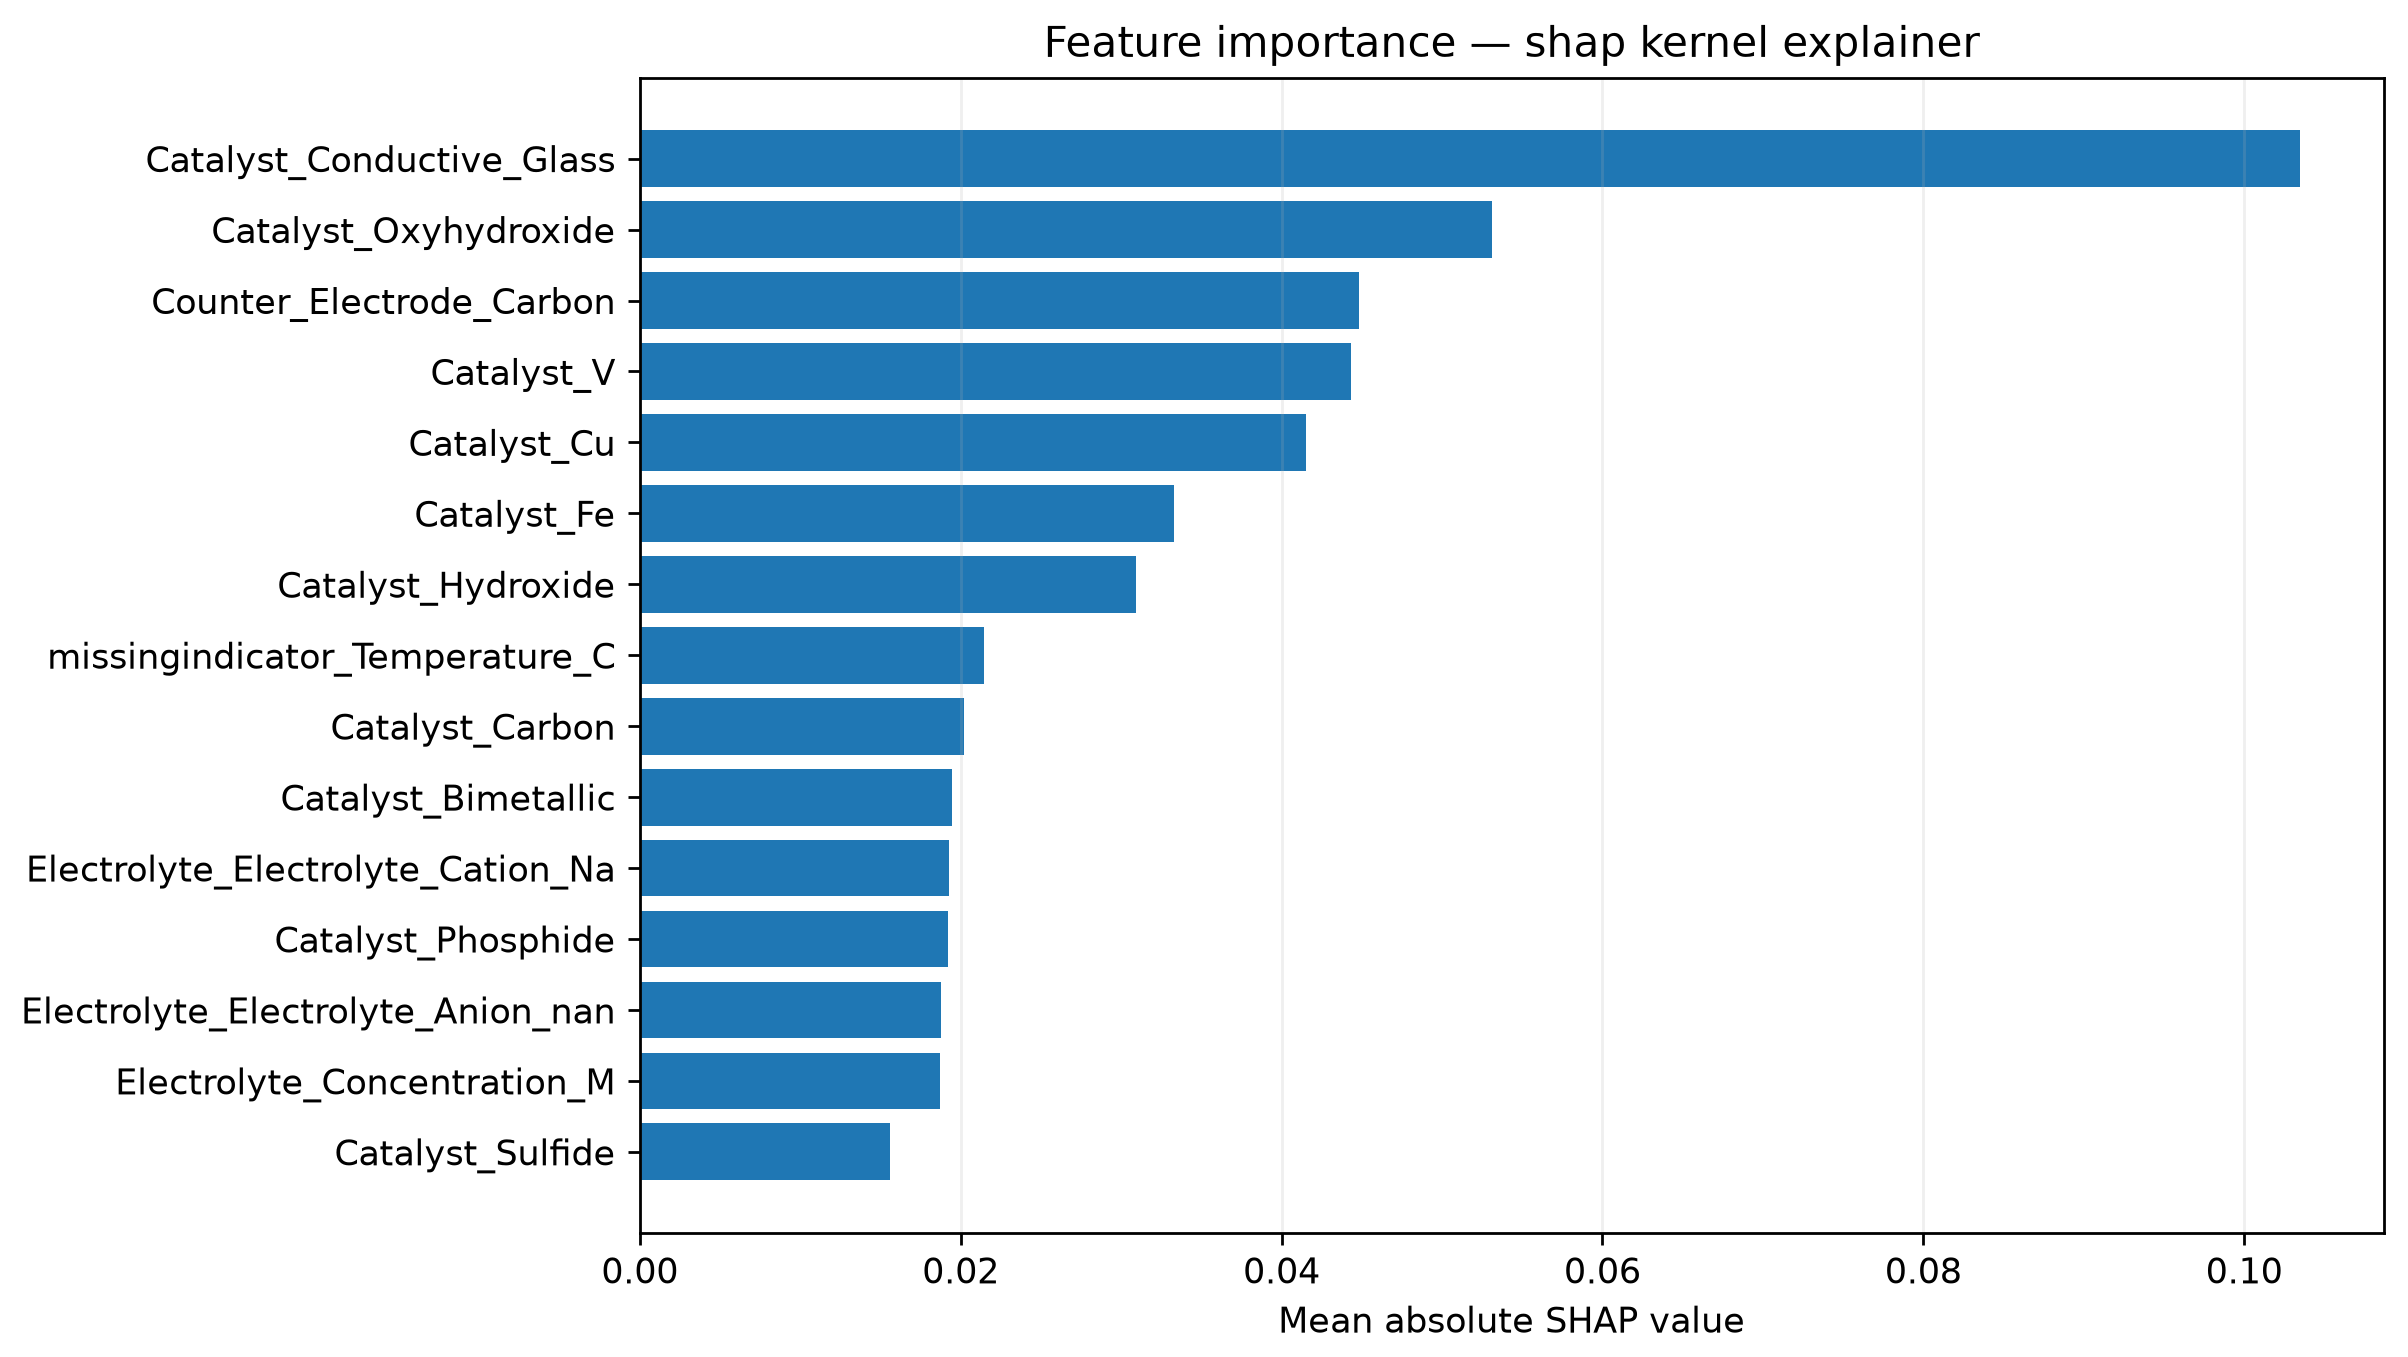
\includegraphics[width=0.8\textwidth,height=0.85\textheight,keepaspectratio]{assets/shap__selected_model_feature_importance.png}
\caption{SHAP feature importance for the selected binary-screen model.}
\label{fig:shapsel}
\end{figure}
\begin{figure}[!htbp]
\centering
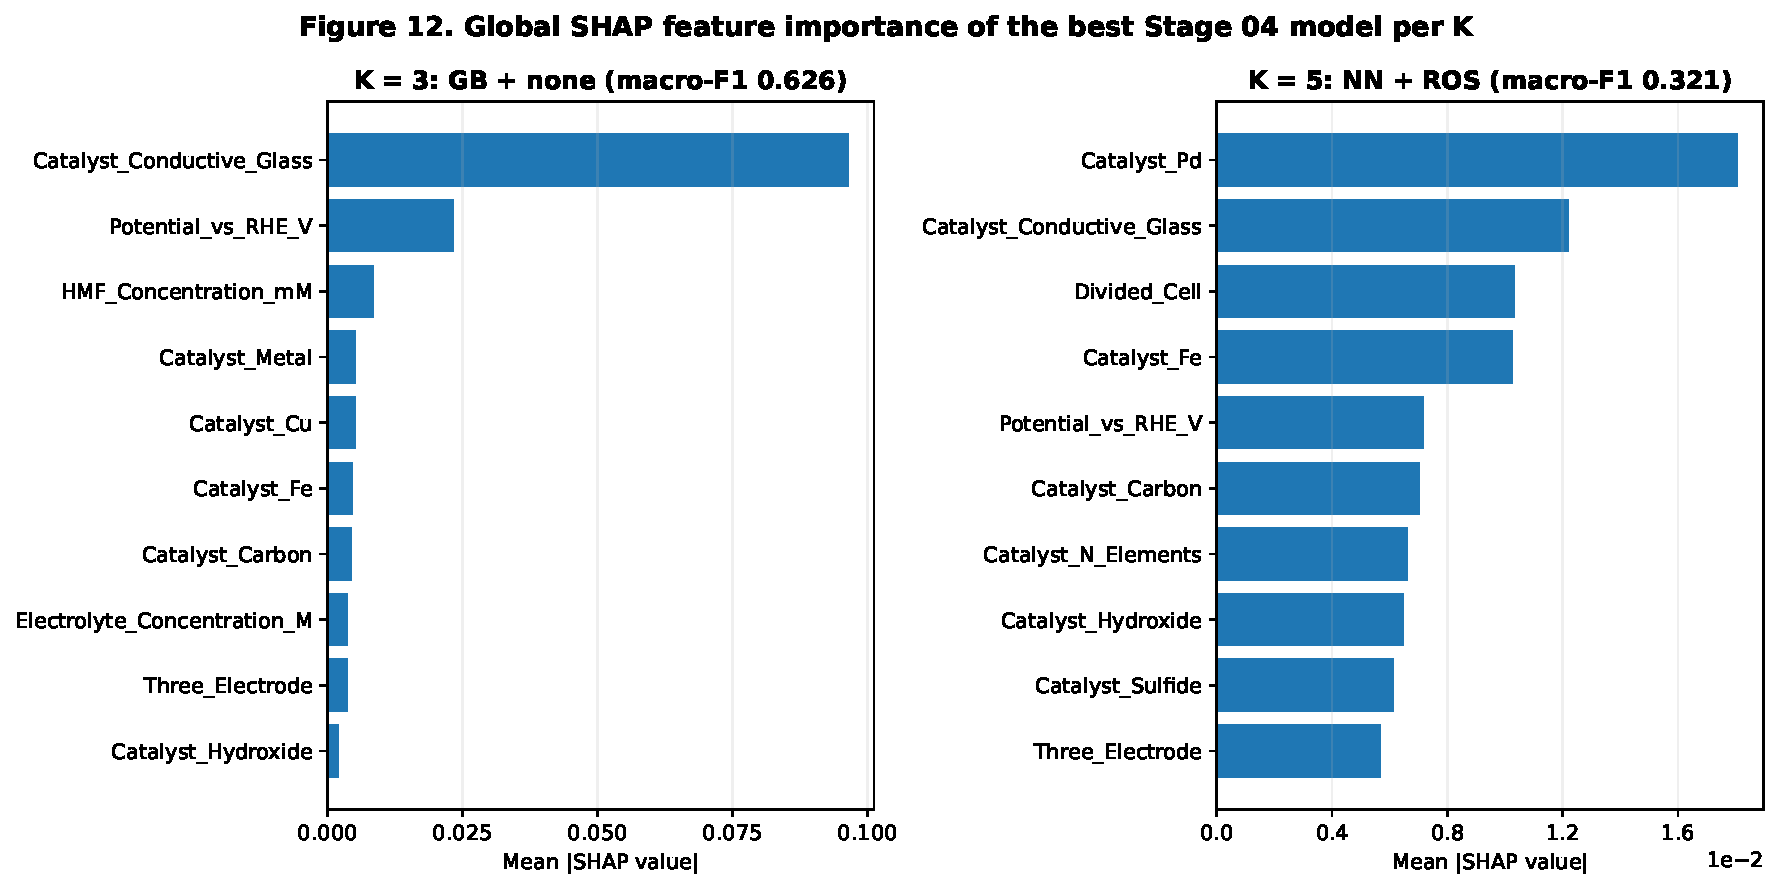
\includegraphics[width=\textwidth,height=0.85\textheight,keepaspectratio]{shap/Figure_12_SHAP_Bar.pdf}
\caption{Global SHAP importance of the best Stage-04 model for $K=3$ and $K=5$.}
\label{fig:fig12}
\end{figure}
\begin{figure}[!htbp]
\centering
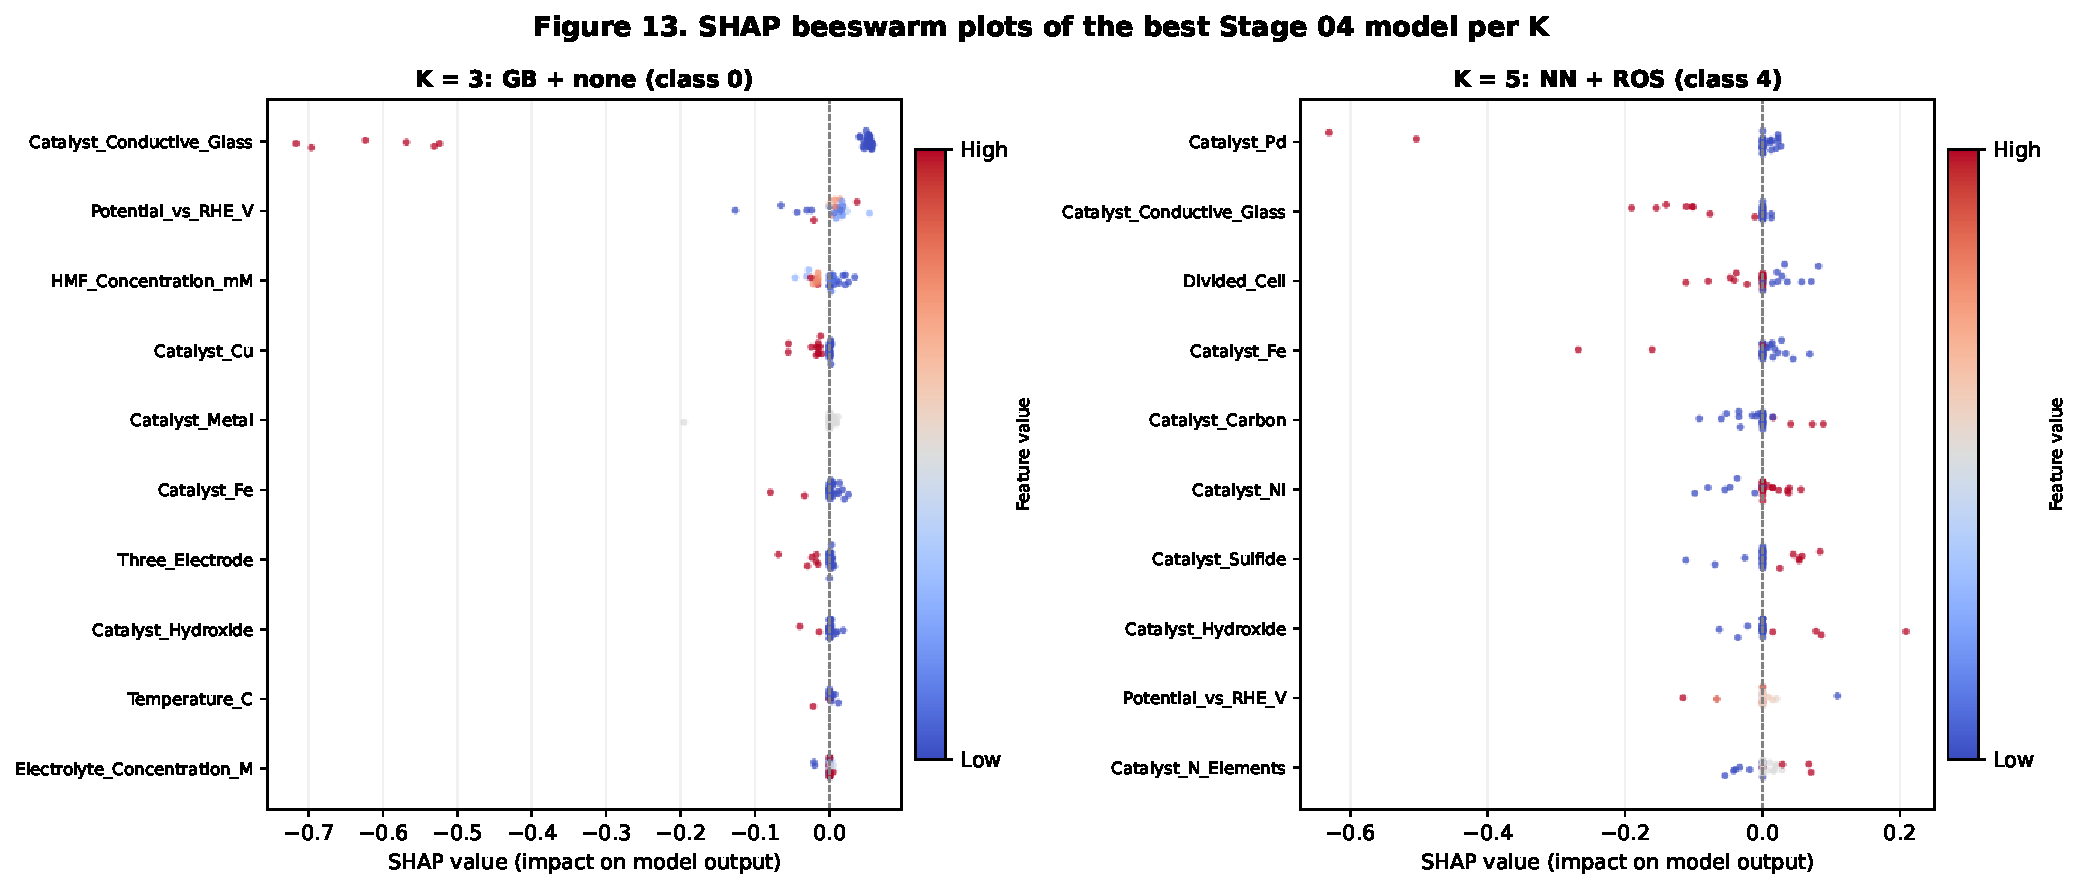
\includegraphics[width=\textwidth,height=0.85\textheight,keepaspectratio]{shap/Figure_13_SHAP_Beeswarm.pdf}
\caption{SHAP beeswarm plots for the majority class at $K=3$ and $K=5$, coloured by feature value.}
\label{fig:fig13}
\end{figure}
\subsection{Regression}
Per-target models reduce MAE relative to the median baseline for all four outcomes (Table~\ref{tab:reg}), but $R^2$ remains between -1.73 and 0.04: the outcome distributions are concentrated near 100\% with a few low outliers, so the models mainly learn to avoid large errors on the typical record rather than to explain variance. The validation gate passed. The joint model trained on the 60 complete records does not beat the baseline (Table~\ref{tab:regjoint}).

\begin{table}[!htbp]
\centering\small
\caption{Per-target regression (primary): publication-grouped cross-validation against a median baseline. MAE and RMSE in percentage points.}
\label{tab:reg}
\begin{tabular}{lrrrrc}
\toprule
Target & $R^2$ & MAE & Baseline MAE & RMSE & Beats baseline \\
\midrule
Conversion & -1.733 & 6.41 & 7.07 & 13.51 & yes \\
Faradaic efficiency & -0.066 & 8.60 & 9.95 & 14.97 & yes \\
Selectivity & 0.030 & 9.97 & 12.37 & 17.20 & yes \\
FDCA yield & 0.044 & 11.86 & 13.19 & 19.50 & yes \\
\bottomrule
\end{tabular}
\end{table}
\begin{table}[!htbp]
\centering\small
\caption{Joint four-output regression on complete rows (secondary): publication-grouped cross-validation against a median baseline. MAE and RMSE in percentage points.}
\label{tab:regjoint}
\begin{tabular}{lrrrrc}
\toprule
Target & $R^2$ & MAE & Baseline MAE & RMSE & Beats baseline \\
\midrule
Conversion & -3.579 & 2.55 & 2.08 & 7.67 & no \\
Faradaic efficiency & -0.376 & 7.28 & 6.89 & 12.43 & no \\
Selectivity & -0.021 & 5.82 & 5.34 & 10.98 & no \\
FDCA yield & -0.049 & 5.74 & 5.29 & 11.11 & no \\
\bottomrule
\end{tabular}
\end{table}
\subsection{Multi-objective optimisation}
NSGA-II (100 individuals, 1000 generations) returned 96 Pareto candidates. Entropy weights for the unconstrained search were: Conversion 0.10, FDCA yield 0.14, Faradaic efficiency 0.18, temperature 0.13, potential 0.45. In the constrained Ni(OH)$_2$/Cu(OH)$_2$ search, all ten top-ranked solutions are Ni(OH)$_2$ on foam, at 0.42--1.10\,M KOH, 1.41--1.42\,V vs RHE and 25--26\,$^\circ$C (Table~\ref{tab:nsga}, Figure~\ref{fig:nsga}). The top candidate's nearest literature record (Ni(OH)2/NF, 1.0 M KOH | 1.45 V vs. RHE) reported 88.3\% yield against 95.2\% predicted; that difference is smaller than the yield regression MAE of 11.9 percentage points. The best Cu(OH)$_2$ candidate is predicted at 91.0\% yield and 94.1\% FE. The spacing metric settles into a stable band after about 20 generations and fluctuates around it thereafter (Figure~\ref{fig:spacing}). Because the predicted gains lie within the regression error, the candidates should be read as experimental starting points, not predictions of record performance.

\begin{table*}[!htbp]
\centering\scriptsize
\caption{NSGA-II top-10 candidates in the constrained Ni(OH)$_2$/Cu(OH)$_2$ search, ranked by entropy-weighted fitness. All performance values are model predictions, not measurements.}
\label{tab:nsga}
\resizebox{\textwidth}{!}{%
\begin{tabular}{rllrrrrrrr}
\toprule
Rank & Catalyst & Electrolyte & HMF (mM) & $E$ (V vs RHE) & $T$ ($^\circ$C) & Conv. (\%) & Yield (\%) & FE (\%) & Fitness \\
\midrule
1 & Ni(OH)2/foam & KOH 1.10\,M & 11.1 & 1.410 & 25.0 & 99.0 & 95.2 & 96.2 & 0.890 \\
2 & Ni(OH)2/foam & KOH 0.80\,M & 12.1 & 1.410 & 25.4 & 99.0 & 95.2 & 96.2 & 0.874 \\
3 & Ni(OH)2/foam & KOH 0.83\,M & 8.2 & 1.411 & 25.2 & 99.0 & 95.4 & 95.0 & 0.866 \\
4 & Ni(OH)2/foam & KOH 0.84\,M & 11.9 & 1.412 & 26.1 & 99.2 & 95.4 & 95.1 & 0.855 \\
5 & Ni(OH)2/foam & KOH 0.45\,M & 11.7 & 1.415 & 25.0 & 99.2 & 94.8 & 94.6 & 0.854 \\
6 & Ni(OH)2/foam & KOH 0.65\,M & 8.8 & 1.412 & 25.7 & 99.2 & 94.9 & 94.7 & 0.851 \\
7 & Ni(OH)2/foam & KOH 0.42\,M & 12.0 & 1.410 & 25.2 & 99.2 & 94.3 & 94.6 & 0.851 \\
8 & Ni(OH)2/foam & KOH 0.69\,M & 11.0 & 1.416 & 25.0 & 99.2 & 94.9 & 94.7 & 0.850 \\
9 & Ni(OH)2/foam & KOH 0.71\,M & 11.5 & 1.412 & 25.5 & 99.2 & 94.5 & 94.9 & 0.844 \\
10 & Ni(OH)2/foam & KOH 0.43\,M & 11.8 & 1.412 & 25.4 & 99.2 & 94.8 & 93.2 & 0.837 \\
\bottomrule
\end{tabular}}
\end{table*}
\begin{figure}[!htbp]
\centering
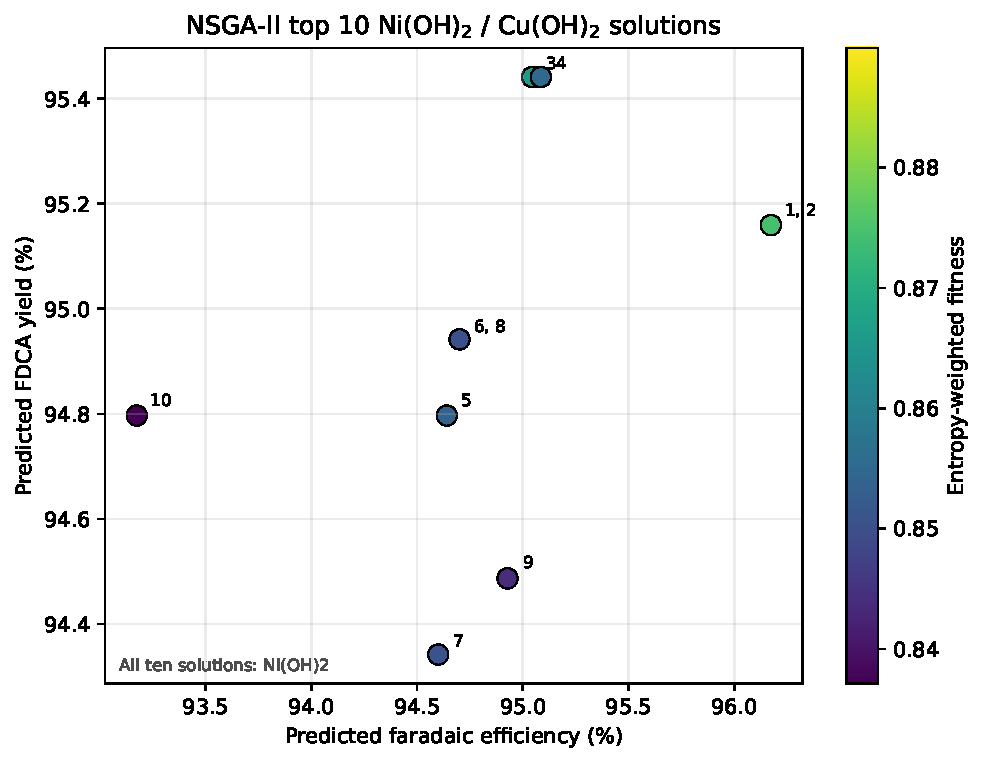
\includegraphics[width=0.75\textwidth,height=0.85\textheight,keepaspectratio]{nsga2/NSGA2_top10_NiCu_hydroxide.pdf}
\caption{Predicted FDCA yield versus FE for the top-10 hydroxide candidates, coloured by entropy-weighted fitness.}
\label{fig:nsga}
\end{figure}
\begin{figure}[!htbp]
\centering
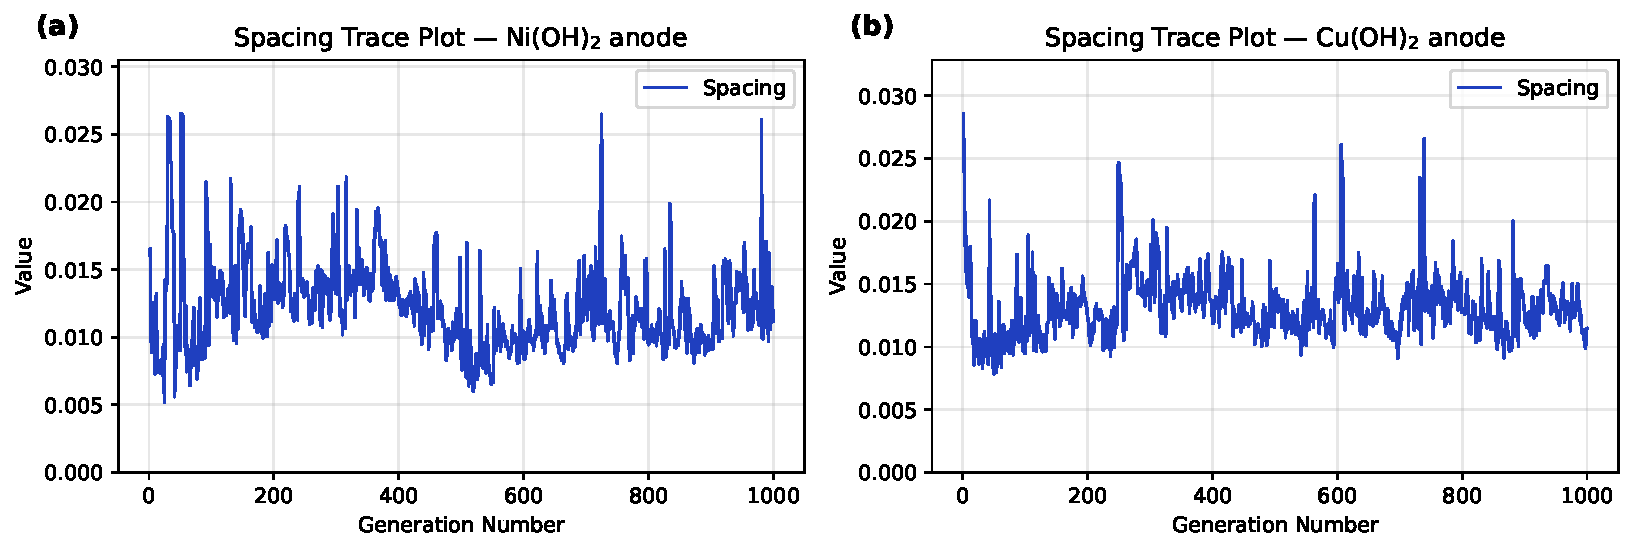
\includegraphics[width=0.75\textwidth,height=0.85\textheight,keepaspectratio]{nsga2/Figure_14_Spacing_Trace.pdf}
\caption{Spacing metric of the first Pareto front over generations.}
\label{fig:spacing}
\end{figure}
\section{Discussion}
\textbf{What improved the scores.} Most of the gain came from data quality rather than model
capacity. Removing counter-electrode contamination and recovering compound families gave the
models chemically meaningful catalyst descriptors; the missing-value indicators restored
information about reporting practice; and disabling early stopping stopped the neural network from
converging on the majority class. Tuning added smaller, family-specific gains.

\textbf{Why 0.76 was not reached.} Several individual repeats of the best binary model exceed 0.76,
but the 25-repeat mean does not. Three factors cap performance: (i) only 119 records from fewer than one hundred papers, many sharing catalysts; (ii) a positive
class that is the majority, so macro-F1 depends heavily on the ~30 low-performance records;
and (iii) between-paper differences in protocol that the descriptors cannot represent. Two
routes would raise the reported number without improving the model: random (non-grouped)
cross-validation, which lets near-duplicate records from one paper appear in training and test,
and redefining the threshold or clusters to suit the classifier. We deliberately did neither.

\textbf{Evaluation lessons.} Silent exclusion of infeasible folds can make a model look several
tenths better than it is; reporting feasibility explicitly is essential when oversampling tiny
classes. Hyperparameters were selected on the same grouped protocol as the reported scores, which
introduces a mild optimistic bias; a nested or external validation set would remove it.

\textbf{Limitations.} Outcomes were imputed for K-means only, so some cluster labels are
pseudo-labels. Descriptors are parsed from free text and remain coarse (no loading, morphology or
surface area). SHAP rankings and NSGA-II candidates are associational and model-dependent.

\section{Conclusions}
A leakage-aware pipeline for literature-scale electrocatalysis data reaches a publication-grouped macro-F1 of 0.731 for a $\geq$90\% performance screen and 0.626 for three-cluster labels, well above chance but short of 0.76. Correct descriptor extraction and honest fold accounting mattered more than model choice. Expanding the corpus, reporting operating conditions completely and validating the NSGA-II candidates experimentally are the most promising next steps.

\section*{Data and code availability}
All results, figures and this manuscript are regenerated by \texttt{python run\_all.py}; this
document is produced by \texttt{scripts/10\_latex\_report.py} from the files in
\texttt{results/} and \texttt{figures/}.

\begin{thebibliography}{9}
\bibitem{li2025} Li \textit{et al.}, \textit{ACS Sustainable Chem.\ Eng.} \textbf{2025}, 13, 13940.
\textcolor{gray}{[Complete author list and title.]}
\bibitem{chawla2002} N.~V. Chawla, K.~W. Bowyer, L.~O. Hall, W.~P. Kegelmeyer, SMOTE: Synthetic
minority over-sampling technique, \textit{J.\ Artif.\ Intell.\ Res.} \textbf{2002}, 16, 321--357.
\bibitem{he2008} H.~He, Y.~Bai, E.~A. Garcia, S.~Li, ADASYN: Adaptive synthetic sampling approach
for imbalanced learning, in \textit{Proc.\ IEEE IJCNN} \textbf{2008}, 1322--1328.
\bibitem{pedregosa2011} F.~Pedregosa \textit{et al.}, Scikit-learn: Machine learning in Python,
\textit{J.\ Mach.\ Learn.\ Res.} \textbf{2011}, 12, 2825--2830.
\bibitem{lemaitre2017} G.~Lema\^{\i}tre, F.~Nogueira, C.~K. Aridas, Imbalanced-learn: A Python
toolbox to tackle the curse of imbalanced datasets in machine learning, \textit{J.\ Mach.\ Learn.\
Res.} \textbf{2017}, 18, 1--5.
\bibitem{lundberg2017} S.~M. Lundberg, S.-I. Lee, A unified approach to interpreting model
predictions, in \textit{Adv.\ Neural Inf.\ Process.\ Syst.} \textbf{2017}, 30, 4765--4774.
\bibitem{deb2002} K.~Deb, A.~Pratap, S.~Agarwal, T.~Meyarivan, A fast and elitist multiobjective
genetic algorithm: NSGA-II, \textit{IEEE Trans.\ Evol.\ Comput.} \textbf{2002}, 6, 182--197.
\end{thebibliography}
\end{document}
